\documentclass{deliverablereport}

\usepackage[style=alphabetic,backend=bibtex]{biblatex}
\addbibresource{report.bib}
\addbibresource{../../lib/publications.bib}

\usepackage{xparse}
\usepackage{etoolbox}
\usepackage{caption}
\graphicspath{{events/}}
 \ExplSyntaxOn

\newcounter{eventcounter}

\newenvironment{event}[7]{
\vspace{0.5cm}
\refstepcounter{eventcounter}
\label{event-#2}
\addcontentsline{toc}{subsection}{\hspace{3ex}-\ Event~\theeventcounter -~ #1}


\noindent\textbf{Event~\theeventcounter -~ #1}\newline % title

\noindent #3 \newline % location and date

\noindent ODK~partners~involved:~ \clist_map_inline:nn{#4}{\site{##1}~}\newline %partners

\ifx&#5&%
      % no participant #
\else
\noindent #5~participants~
\ifx&#6 &%
    % no odk participant
\else 
~(including~#6~from~within~ODK)\newline
\fi
\fi

\ifx&#7&%
      % no website
\else
\noindent \url{#7}\newline
\fi



}{\begin{center}\noindent\rule{4cm}{0.4pt}\end{center}}

 \ExplSyntaxOff


\deliverable{dissem}{workshops-3}
\duedate{31/08/2018 (M36)}
\deliverydate{08/09/2018}
\author{Viviane Pons et al.}

\begin{document}
\maketitle
\githubissuedescription
\newpage
\tableofcontents
\newpage

\section{Development workshops}

We call a development workshop an event with a restricted number of participants
who meet to work on a specific task. These workshops are an inherent part
of \ODK development process as described in \taskref{dissem}{devel-workshops}:
 they bring together
developers from within and outside of \ODK and allow effective work
and discussions on many technical aspects. They also participate in building
and maintaining a community of developers inside \ODK and within the
open-source communities we belong to.

Throughout years 2 and 3 of the project, we have had 15 workshops dedicated mostly
to development. Some of them also included a training approach. 

\subsection{Ateliers PARI-GP}

The PARI/GP Ateliers were established in 2012 as a yearly meeting
between developers and users of the PARI/GP system.

The main goals are advertising new features and improvements,
discussing further developments, sharing best practices, and collaborative
code writing (hacking sessions, doc reviews, bug-squashing parties).

You can find the list of previous PARI Ateliers at
\url{http://pari.math.u-bordeaux.fr/ateliers.html}.

We have listed here the three Ateliers which focused more on development. 
Other Ateliers can be found under the Dissemination section.

\begin{event}{Atelier PARI/GP 2017}{AtelierPARI2017}{Grenoble (FR),
2017-01-09 to 2017-01-13}{PS,UB,UV,UW}{36}{http://pari.math.u-bordeaux.fr/Events/PARI2017/}

\textbf{Main goals.}

The PARI/GP Ateliers were established in 2012 as a yearly meeting
between developers and users of the PARI/GP system.

The main goals are advertising new features and improvements,
discussing further developments, sharing best practices, and collaborative
code writing (hacking sessions, doc reviews, bug-squashing parties).

You can find the list of previous PARI Ateliers at
\url{http://pari.math.u-bordeaux.fr/ateliers.html}

\textbf{ODK implication.} 
%Describe how ODK was involved and give a rough estimation of cost for ODK

\ODK participants: B. Allombert, K. Belabas, V. Delecroix, J. Demeyer,
J.-P. Flori, L. de Feo.

\ODK provided the main funding source for the workshop (accommodation,
subsistence and travel expenses), for about XXXk\euro. The Lyon
institute of mathematics (Institut Camille Jordan) co-funded the event.

\textbf{Event summary.} 
%Give a summary of your event

The 7th Atelier PARI/GP took place in Lyon (France) from january
9th to 13th.

There were 43 registered participants from 19 different institutions
(no registration fees).

A typical day of the workshop had introductory talks and tutorials
in the morning; afternoons allowed ample time for hacking sessions,
discussions and training.

The Atelier featured 10 morning talks on mathematical topics and
implementation projects including 4 talks by ODK members
\begin{itemize}
\item Karim Belabas ``Using GIT with PARI'', ``$L$-functions'' and
  ``Dirichlet characters''
\item Bill Allombert ``New GP features''
\end{itemize}

Slides for all talks are available at
\url{http://pari.math.u-bordeaux.fr/Events/PARI2017/}

\textbf{Results and impact.} 
% What did you achieve with this event? (If ever it impacted 
% other ODK tasks and deliverables, mention it here)

The workshop was very productive and particularly beneficial to WP5
(high-performance computing). It also was a successful dissemination event: half
  the participants had not come to a previous Atelier.

\end{event}


\begin{event}{Atelier PARI/GP 2017b}{AtelierPARI2017b}{Clermont-Ferrand (FR),
2017-06-19 to 2017-06-23}{PS,UB,UV,UW}{36}{3}{http://pari.math.u-bordeaux.fr/Events/PARI2017b/}


\textbf{ODK implication.} 
%Describe how ODK was involved and give a rough estimation of cost for ODK

\ODK participants: B. Allombert, K. Belabas, J.-P. Flori

\ODK provided the main funding source for the workshop (accommodation,
subsistence and travel expenses), for about 12k\euro. The following
institutions co-funded the event through Clermont institute of mathematics
  (Laboratoire
  Blaise Pascal): GDR Structuration de la Théorie des Nombres (CNRS), Région
  Auvergne Rhône-Alpes, Conseil départemental Puy-de-Dôme, Université
  Auvergne-Rhônes-Alpes and the city of Clermont-Ferrand.

\textbf{Event summary.} 
%Give a summary of your event

The 8th Atelier PARI/GP took place in Clermont-Ferrand (France) from june
19th to 23rd with a special focus on Elliptic curves, Modular Forms and
$L$-Functions.

There were 36 registered participants from 16 different institutions
(no registration fees).

A typical day of the workshop had introductory talks and tutorials
in the morning; afternoons allowed ample time for hacking sessions,
discussions and training.

The Atelier featured 13 morning talks.

\textbf{Results and impact.} 
% What did you achieve with this event? (If ever it impacted 
% other ODK tasks and deliverables, mention it here)
This was a dissemination event with a special focus on recently developped
packages (Elliptic curves over number fields, Modular forms), before they were
merged into a formal release. We got lots of feedback on the interface and
documentation and a number of bugs and glitches were fixed as a result.
\end{event}


\begin{event}{Atelier PARI/GP 2018}{AtelierPARI2018}{Besan\c{c}on (FR),
2018-01-15 to 2017-01-19}{PS,UB,UV,UW}{36}{6}{http://pari.math.u-bordeaux.fr/Events/PARI2018/}

\textbf{Main goals.}

The PARI/GP Ateliers were established in 2012 as a yearly meeting
between developers and users of the PARI/GP system.

The main goals are advertising new features and improvements,
discussing further developments, sharing best practices, and collaborative
code writing (hacking sessions, doc reviews, bug-squashing parties).

You can find the list of previous PARI Ateliers at
\url{http://pari.math.u-bordeaux.fr/ateliers.html}

\textbf{ODK implication.} 
%Describe how ODK was involved and give a rough estimation of cost for ODK

\ODK participants: B. Allombert, K. Belabas, V. Delecroix, J. Demeyer,
J.-P. Flori, L. de Feo.

\ODK provided the main funding source for the workshop (accommodation,
subsistence and travel expenses), for about 13k\euro. The Besan\c{c}on
institute of mathematics co-funded the event.

\textbf{Event summary.} 
%Give a summary of your event

The 10th Atelier PARI/GP took place in Lyon (France) from january
15h to 19th.

There were 38 registered participants from 19 different institutions
(no registration fees).

A typical day of the workshop had introductory talks and tutorials
in the morning; afternoons allowed ample time for hacking sessions,
discussions and training.

The Atelier featured 8 morning talks on mathematical topics and
implementation projects including 4 talks by ODK members
\begin{itemize}
\item Karim Belabas ``Modular Forms''
\item Bill Allombert ``New GP features'', \texttt{lfun} and Artin
  $L$-functions.
\item Luca de Feo and Jean-Pierre Flori ``Algorithms for lattices of
  compatibly embedded finite fields''.
\end{itemize}

Slides for all talks are available at
\url{http://pari.math.u-bordeaux.fr/Events/PARI2018/}

\textbf{Results and impact.} 
% What did you achieve with this event? (If ever it impacted 
% other ODK tasks and deliverables, mention it here)

The workshop was very productive and particularly beneficial to WP5
(high-performance computing), it provided final feedback on recent PARI/GP
  modules and interfaces that paved the way for the release of
  pari-2.10-alpha (2018/05) and pari-2.11-stable (2018/07, the first major
  release since 2016).
  
It also was a successful dissemination event: 14 participants had not come to
  a previous Atelier.
\end{event}


\subsection{Linbox meetings}

The LinBox developer meeting are meant to gather developers and users of the
LinBox ecosystem (composed of \texttt{givaro}, \texttt{fflas-ffpack} and
\texttt{LinBox}).

The main goals are to enable interactions between the several groups of
developers and users in order to share experiences, take collegiate design
decisions and practice collaborative code writing.

\begin{event}{LinBox Days December 2017}{LinBoxDays17}{Camaret sur Aigue (FR),
2017-12-13 to 2017-12-15}{UGA}{9}{3}{https://github.com/linbox-team/fflas-ffpack/wiki/LinBox-developper-meeting-in-Camaret}

\textbf{Main goals.}

The LinBox developper meeting are meant to gather developper and users of the
LinBox ecosystem (composed of \texttt{givaro}, \texttt{fflas-ffpack} and
\texttt{LinBox}).

The main goals are to enable interraction between the several groups of
developpers and users in order to share experiences, take collegial design
decision and practice collaborative code writing.

\textbf{ODK implication.} 
%Describe how ODK was involved and give a rough estimation of cost for ODK

\ODK participants: C. Pernet, J.-G. Dumas, H. Zhu.

\ODK provided the main funding source for the workshop (accommodation,
subsistence and travel expenses), for about 2.1k\euro.

\textbf{Event summary.} 
%Give a summary of your event

The Camaret LinBox developper meeting took place in Grignan (France), from December
13th to 15th, 2017.

There were 9 participants from 3 different institutions (UGA, Université
Montpellier 2, US Naval Academy).
No registration fees were applied.

After a round table branstorming on developpment projects for the meeting,
developpers gathered in groups each adressing a given project.
The main achievements of the meeting include
\begin{itemize}
\item Progress on the distributed parallel ration solver (\delivref{hpc}{LinBox-distributed});
\item Improvement on the polynomial matrix algorithmic;
\item wider support of SIMD micro-architectures;
\item Cleanup and simplification of the build system;
\item Improvement of code robstness and release preparation (\delivref{hpc}{LinBox-algo}).
\end{itemize}


\textbf{Results and impact.} 
% What did you achieve with this event? (If ever it impacted 
% other ODK tasks and deliverables, mention it here)

The workshop was very productive and particularly beneficial to WP5
(\delivref{hpc}{LinBox-algo} and \delivref{hpc}{LinBox-distributed}).
\end{event}


\begin{event}{LinBox Days June 2018}{LinBoxDays18}{Grignan (FR),
2018-06-20 to 2018-06-22}{UJF}{9}{3}{https://github.com/linbox-team/fflas-ffpack/wiki/LinBox-developper-meeting-in-Grignan}

\textbf{Main goals.}

The LinBox developper meeting are meant to gather developper and users of the
LinBox ecosystem (composed of \texttt{givaro}, \texttt{fflas-ffpack} and
\texttt{LinBox}).

The main goals are to enable interraction between the several groups of
developpers and users in order to share experiences, take collegial design
decision and practice collaborative code writing.

\textbf{ODK implication.} 
%Describe how ODK was involved and give a rough estimation of cost for ODK

\ODK participants: C. Pernet, J.-G. Dumas, H. Zhu.

\ODK provided the main funding source for the workshop (accommodation,
subsistence and travel expenses), for about 2.6k\euro.

\textbf{Event summary.} 
%Give a summary of your event

The Grignan LinBox developper meeting took place in Grignan (France), from June
20th to 22nd.

There were 9 participants from 3 different institutions (UGA, Université
Montpellier 2, US Naval Academy).
No registration fees were applied.

After a round table branstorming on developpment projects for the meeting,
developpers gathered in groups each adressing a given project.
The main achievements of the meeting include
\begin{itemize}
\item Progress on the distributed parallel ration solver (\delivref{hpc}{LinBox-distributed});
\item Design and refactorization of the code for randomized algorithms in LinBox;
\item Completion of the rewrite of the prime fields in Givaro;
\item Improvement of code robstness and release preparation (\delivref{hpc}{LinBox-algo}).
\end{itemize}


\textbf{Results and impact.} 
% What did you achieve with this event? (If ever it impacted 
% other ODK tasks and deliverables, mention it here)

The workshop was very productive and particularly beneficial to WP5 (\delivref{hpc}{LinBox-algo}).
\end{event}


\subsection{Jupyter meetings}

\begin{event}{Jupyter Widgets Workshop}{JupyterWidget}{École Polytechnique, January 23-26}{PS,SR,UG}{27}{3}{https://github.com/OpenDreamKit/OpenDreamKit/issues/246}

\textbf{Main goals.} Bringing together developers and power users of Jupyter Widgets.

\textbf{ODK implication.} Some organizational support; funding of ODK participants; \approx 1k€.

\textbf{Event summary.} This was the first workshop specifically
centered on Jupyter widgets. If featured tutorials on how to implement
widgets, demonstrations of widget uses for 3D visualization and big
data analysis, improvements of core widget functionalities for better
integration, and implementation of new widgets. In addition the
workshop was the occasion to advance other Jupyter related task in
\ODK's WorkPackage 4.

\textbf{Results and impact.} The intense cross-interactions between
developers from academia, Jupyter-centric SMÉ's, and big institutions
(banks, US military) highlighted and further pushed the wide adoption
of this technology and the building of a community around it.
\end{event}

\begin{event}{JupyterHub and Binder coding sprint}{JupyterHub}{Université Paris Sud, March 7-8}{PS,SR,LL}{8}{4}{https://pad.unistra.fr/p/jupyterhub-dev}

  \textbf{Main goals.} This event was organized as a satellite of a
  Jupyter dissemination conference at École Polytechnique. It brought
  together developers of the Virtual Environments JupyterHub and
  BinderHub and DevOps working on deployments in Orsay and at EGI for
  a coding sprint. The goal was to improve those deployments, as a use
  case from which to learn and share procedures and best practices.

  \textbf{ODK implication.} Organization and funding of ODK participants; $\approx$ 1k\euro.

  \textbf{Results and impact.} Turnkey deployment instructions already
  existed for deploying JupyterHub and BinderHub on top of cloud
  infrastructure provided by e.g. Google Cloud, or Microsoft Azure.
  This workshop was a major step for the first deployment of a
  JupyterHub and BinderHub instance on top of an OpenStack cloud
  infrastructure. This is important as OpenStack is widely adopted in
  academia-run cloud infrastructures, yet raises some unique
  challenges due to its high customizability. Many notes were taken
  and shared. In addition a blog post summarized a brainstorm on the
  upcoming convergence between JupyterHub and BindherHub, toward
  providing versatile JupyterHub deployments that lets its user
  define, run, and share virtual environments equipped with an
  arbitrary software stack.

  \url{https://opendreamkit.org/2018/03/15/jupyterhub-binder-convergence/}
\end{event}


\subsection{Cross-project meetings}

As the project evolves, we are prone to have more and more events which 
concern many software projects altogether. All the 10 events below
included members from various communities to work on interactions and
general cross-projects technical questions. This included two special
workshops at ICMS 2018 as well as events at CICM 2017 and 2018.

\begin{event}{Sage/GAP Days 85: packaging, portability, documentation tools}{sd85}{Cernay (France) 2017-03-13 to 17}{PS,UV,UG,SA,UB}{15}{9}{https://wiki.sagemath.org/days85}

  \textbf{Main goals.} This developer meeting was focused on
  initiating long term work on ODK tasks related to packaging,
  portability and documentation tools for GAP and SageMath.

  \textbf{ODK implication.} This event was organized and funded by
  \ODK (Paris Sud).

  \textbf{Event summary.} An intensive week with many brainstorms and coding sprints.

  \textbf{Demographic.} 9 ODK members from five sites together with
  half a dozen other participants

  \textbf{Results and impact.} Proper packaging and distribution has
  been a recurrent issue for large computational software like \Sage
  or \GAP, and is a major task for ODK
  (\longtaskref{component-architecture}{mod-packaging}). This workshop
  was a follow up to the highly successful \Sage Days 77 organized in
  2016 by \ODK where long term plans were designed. Here the workshop
  focused on accelerating the implementation of the plans, with highly
  productive collaborative coding sprints on topics such as \GAP and
  \Sage packaging (Conda, ...), \Sage portability (Windows) and
  documentation, \GAP's build system and release management, and how
  to best integrate \GAP and \Sage together via a shared library.
\end{event}


\begin{event}{Live Structured Documents}{live-documents}{Location and date}{SR,PS,FAU}{11}{6}{https://www.eventbrite.com/e/opendreamkit-workshop-on-live-structured-documents-registration-37364670736}

\textbf{Main goals.} To facilitate development of live structured documents, using Jupyter infrastructure, such as interactive documentation and publication.

\textbf{ODK implication.}
The workshop was hosted at \ODK site, Simula Research Laboratory in Oslo, Norway. The only cost to \ODK was travel reimbursements to bring five participants to Oslo, Norway for three days.

\textbf{Event summary.} The event was a workshop gathering \ODK participants and others interested in interactive documents of various kinds.
Participants discussed available technologies and goals,
and worked together to build tools in this area,
especially collaborating to integrate across projects with different stakeholders.

\textbf{Results and impact.}
One of the main impacts of the workshop
was the creation of a new package, \href{https://github.com/minrk/thebelab}{thebelab},
which builds on \Jupyter technology
to add interactive code execution to any webpage,
with execution running on \href{https://mybinder.org}{mybinder.org} or a local \Jupyter server.
During the workshop, thebelab was put to use in \href{https://more-sagemath-tutorials.readthedocs.io/en/latest/}{documentation for
SageMath} and tested with documentation for both Singular and GAP.
This serves WP4 by adding the possibility of interactivity to documentation for projects in the \ODK community,
and benefiting from kernels for GAP and other \ODK projects developed in T4.1,
showing the value of integrating \ODK systems into a shared \Jupyter ecosystem.

\end{event}


\begin{event}{Workshop on interfacing (math) software with low level libraries}{Cernay 2018}{Cernay (France) 2018-04-30 to 2018-05-04}{PS,CNRS,UV,UGent,LL}{15}{https://github.com/OpenDreamKit/OpenDreamKit/issues/251}

  \textbf{Main goals.} This developer meeting was focused on
  initiating long term work on ODK tasks related to packaging,
  portability and documentation tools for SageMath.

  \textbf{ODK implication.} This event was organized and funded by
  \ODK (Paris Sud).

  \textbf{Event summary.} An intensive week with some short informal
  presentations, and many brainstorms and coding sprints.

  \textbf{Demographic.} 11 ODK participants from five sites together
  with 14 other experts of a variety of systems such as Oscar,
  Polymake, CERN's Root, Cython, Jupyter and C++, Numba, Dask,
  libsemigroups,

  \textbf{Results and impact.} (Math) Computational systems face a
  tension between using high level languages (e.g. Python) for
  expressivity, ease of use and prototyping, and low-level languages
  (e.g. C/C++) for power and speed, and also for modularity (using
  existing libraries, or writing reusable ones). To resolve this
  tension, many approaches have been explored in the recent years, and
  the frontier between the two worlds is becoming increasingly blurry.

  This workshop brought together developers from a large variety of
  horizons to share expertise, seek collaboration venues, and get into
  concrete action. This was quite bold of an aim.

  The format was informal and flexible, with presentations and
  tutorials to let information flow, and lots of time for coding
  sprints. This was very productive, as testified by the exit survey:
  to the question “Would you recommend to your colleagues to attend a
  workshop with this format”, 9 answers were ``yes definitely'' ad the
  other two ``yes''; a participant well outside of ODK's usual scope
  wrote as testimony «The looseness made it more productive than any
  workshop I've ever attended».

  Notes were taken collectively with the eventual aim to author a
  joint survey of the available technologies and best practices; the
  current draft is available from
  \url{https://www.overleaf.com/read/wrmkhfvwmxnz}.
\end{event}


\begin{event}{GAP Days -- Jupyter in GAP and other CAS}{GAPDAYS2018}{St Andrews, United Kingdom, 4th to 8th June 2018}{SA}{13}{4}{https://www.gapdays.de/gap-jupyter-days2018}

  \textbf{Main goals.} The aim of the workshop was to bring together
  developers and early adopters of Jupyter, Binder, Thebelab and other
  web technology relevant for Virtual Environments for research and
  teaching, with some focus on the GAP computational system.

Topics that were worked on included:

\begin{itemize}
\item The GAP JupyterKernel
\item Javascript-Visualizations using Jupyter
\item Using Thebe for interactive manuals
\item Developing teaching materials with Jupyter, and publishing them using MyBinder
\item Writing academic publications using MyBinder and Docker images, to make
  all computational results and all examples fully and easily reproducible.
\item Discussing demands on software and hardware infrastructure in day to day
  use.
\end{itemize}


\textbf{\ODK implication.} Organised by Markus Pfeiffer at UStan. \ODK paid for
the workshop dinner, the accommodation for Nusa Zidaric, Pedro
Garcia-Sanchez, and Sergio Siccha, travel and accommodation for Nicolas Thiéry.


\textbf{Event summary.} We met in a small group of developers and interested
clients of our Jupyter, ThebeLab, Binder and other web technology relevant for
virtual research environments, focused on GAP and the wider context of
OpenDreamKit. We explained how the GAP Jupyter Kernel works, developed some
prototypes with and improvements of the GAP Jupyter kernel.
%
We demonstrated the work of Manuel Martins (Markus Pfeiffer's PhD student),
Sebastian Gutsche, and Pedro A. García-Sánchez who are using GAP's Jupyter
kernel in research and teaching and to develop new ways of using them.

% The event consisted of the following talks
% \begin{itemize}
% \item \emph{Introduction to the GAP-Jupyter kernel} -- Markus Pfeiffer (University of St Andrews),
% \item \emph{Basic setup for Binder} -- Sebastian Gutsche (University of Siegen),
% \item \emph{ThebeLab demo} -- Nicolas M. Thiéry (Paris Sud),
% \item \emph{Experiencing with Jupyter GAP} -- Pedro Garcia-Sanchez (Universidad de Granada),
% \item \emph{FSR - Feedback Shift Registers} -- Nusa Zidaric (University of Waterloo).
% \end{itemize}

To structure programming work and discussions, we followed the well-established
practice of a stand-up meeting in the morning to coordinate work, and a meeting
in the afternoon to record achievements.
%
Discussions ranged from deepining the understanding of how Jupyter works, and
what needs the research and teaching community has to more technical topics
which reach into other workpackges such as improved integration between SageMath
and GAP.

\textbf{Results and impact.} Teachers and researchers intending to use the GAP
Jupyter kernel and adjacent technologies in teaching and research, are now much
more comfortable using these technologies. The demonstration of the
possibilities left a good impression of the potential of this technology.

% The workshop was very productive. The goal of a readily packaged JupyterKernel
% for GAP was achieved, an improved Docker deployment of GAP has been provided.
% Apart from work on WP4, we also achieved progress on WP3 and WP6 through
% discussions and indentification of synergies between the software demands of
% these workpackages.


\end{event}


\subsection{\ODK project meeting}

\begin{event}{Project meeting in XFEL}{PMxfel}{XFEL Hamburg, June 20 --22, 2018}{XFEL, PS, LL, UW, LEEDS, SR, US, UK}{13}{13}{https://opendreamkit.org/2018/06/20/Hamburg-DisseminationWorkshop-SteeringMeeting/}

\textbf{Main goals.} At the occasion of the project meeting, we also held a workshop on dissemination and a Jupyter workshop on 3d graphics.

\textbf{ODK implication.} The event was hosted by XFEL and each participant was funded by ODK through their institutions.

\textbf{Event summary.} The first part of the event was focused on dissemination and communication in ODK. It was an occasion to expose what had been done in the previous years and start a reflexion on how to better promote it. We discussed the new website design and organization and we wrote some new content. We also had a professional interviewer on site who conducted interviews of the ODK team to give an overview of the project goals, accomplishments, and philosophy. The second part of the event was dedicated to a Jupyter workshop on 3d graphics.

\textbf{Demographic.} All participants were ODK members.

\textbf{Results and impact.} This was a very useful consultation. The new website was released in the following weeks. The interviews are still being edited but should be live soon.


\end{event}



\section{Dissemination and outreaching activities}

We describe here all activities related to \taskref{dissem}{dissemination}:
these are all events oriented towards dissemination, training, and outreach. This
includes events organized or co-organized by \ODK and also
participating in external events and many communication activities.

\subsection{Training workshops and events}

Training the community to use the tools developed by \ODK has become a big 
part of our work. By organizing specific workshops, or events inside bigger
conferences, \ODK members have been able to share \ODK technologies such as \Jupyter,
\Sage, \GAP, PARI-GP with more than 500 end users.

\begin{event}{Second CoDiMa Training School in Computational Discrete Mathematics}{codima2016}{ICMS, Edinburgh, Oct. 17 -- 21, 2017}{SA,USH,UW,PS}{38}{6}{https://www.codima.ac.uk/school2016/}

\textbf{Main goals.} This training school was organised for PhD students and researchers from
UK institutions interested in using computational techniques in the area of discrete mathematics.
The aim was to give an introduction into open source mathematical software packages in this area,
at the same time equipping attendees with modern skills that they need for using and developing
research software, and promoting best open science practices.

\textbf{\ODK implication.} The school has been organised by Alexander Konovalov (USTAN) and supported
by the EPSRC-funded project CoDiMa (CCP in the area of Computational Discrete Mathematics). Presenters
included Alexander Konovalov, Steve Linton and Markus Pfeiffer (USTAN), Viviane Pons (UPSud),
Mike Croucher (USFD) and John Cremona (UWarwick).

\textbf{Event summary.}

It started with the hands-on Software Carpentry workshop covering basic
concepts and tools, including working with the command line, version control and task automation,
continued with introductions to GAP and SageMath systems, and followed by the series of lectures
and exercise classes on a selection of topics in computational discrete mathematics. Alexander
Konovalov gave an introduction to GAP in the form of the Software Carpentry lesson. It was
followed by Steve Linton's talk ``How to use GAP effectively'' and Markus Pfeiffer's talks
``Advanced GAP programming'' and ``Pathways to impact : contributing to GAP''.
Viviane Pons gave a SageMath tutorial, and John Cremona presented LMFDB project.
Other speakers were Christopher Jefferson (St Andrews) with
``Debugging and profiling in GAP'' and
``Building Efficient Algorithms on Permutation Groups with Stabilizer Chains''
and Wilf Wilson (St Andrews) with ``Semigroups in GAP: an introduction and tutorial''.
Both Markus Pfeiffer and Wilf Wilson used GAP Jupyter interface in their talks.
The closing activities were the talk ``Is your research software correct?'' by Mike Croucher
and a panel discussion joined by the director of the Software Sustainability Institute Neil Chue Hong.

\textbf{Demographic.} There were 10 women among 26 learners attending the School.

\textbf{Results and impact.} This event contributed to building UK community
around \ODK components, and to dissemination of \ODK outputs in the UK.

\end{event}


\begin{event}{Computational Mathematics with Jupyter}{ICMS-Jupyter}{ICMS, Edinburgh, Jan. 16 -- 20, 2017}{SA,PS,USH,UO,USO,UW,LL,SR,UG}{47}{20}{https://opendreamkit.org/meetings/2017-01-16-ICMS/}

\textbf{Main goals.} The focus of the workshop was on various components from the Jupyter's ecosystem 
and related projects such as, for example, Jupyter notebooks kernels for mathematical software systems,
and their applications in research, training and teaching.

\textbf{ODK implication.} The workshop has been organised by Alexander Konovalov and Markus
Pfeiffer (USTAN). OpenDreamKit speakers included Marijan Beg, Mike Croucher, Jeroen Demeyer,
Hans Fangohr, Vidar Fauske, Alexander Konovalov and Markus Pfeiffer. Many other ODK members
were attending and took part in various activities taking place during the workshop.
The full list of participants is available at
\url{https://opendreamkit.org/meetings/2017-01-16-ICMS/participants/}.
The costs primarily included catering during the workshop and travel expenses.
Some expenses were covered by our partner project CoDiMa which supports computational
discrete mathematics community in the UK.

\textbf{Event summary.}

The workshop combined presentations and tutorials (mainly during morning sessions)
with concurrent coding and documentation sprints, which were advertised to the participants
to sign up. At the end of each day we heard brief reports from group activities.
The programme of the workshop is available
at \url{https://opendreamkit.org/meetings/2017-01-16-ICMS/programme/}. A very detailed
summary of the even is given by Raniere Silva (Software Sustainability Institute) and
Hans Fangohr at \url{https://www.software.ac.uk/blog/2017-02-07-computational-mathematics-jupyter}.

\begin{figure}[ht]
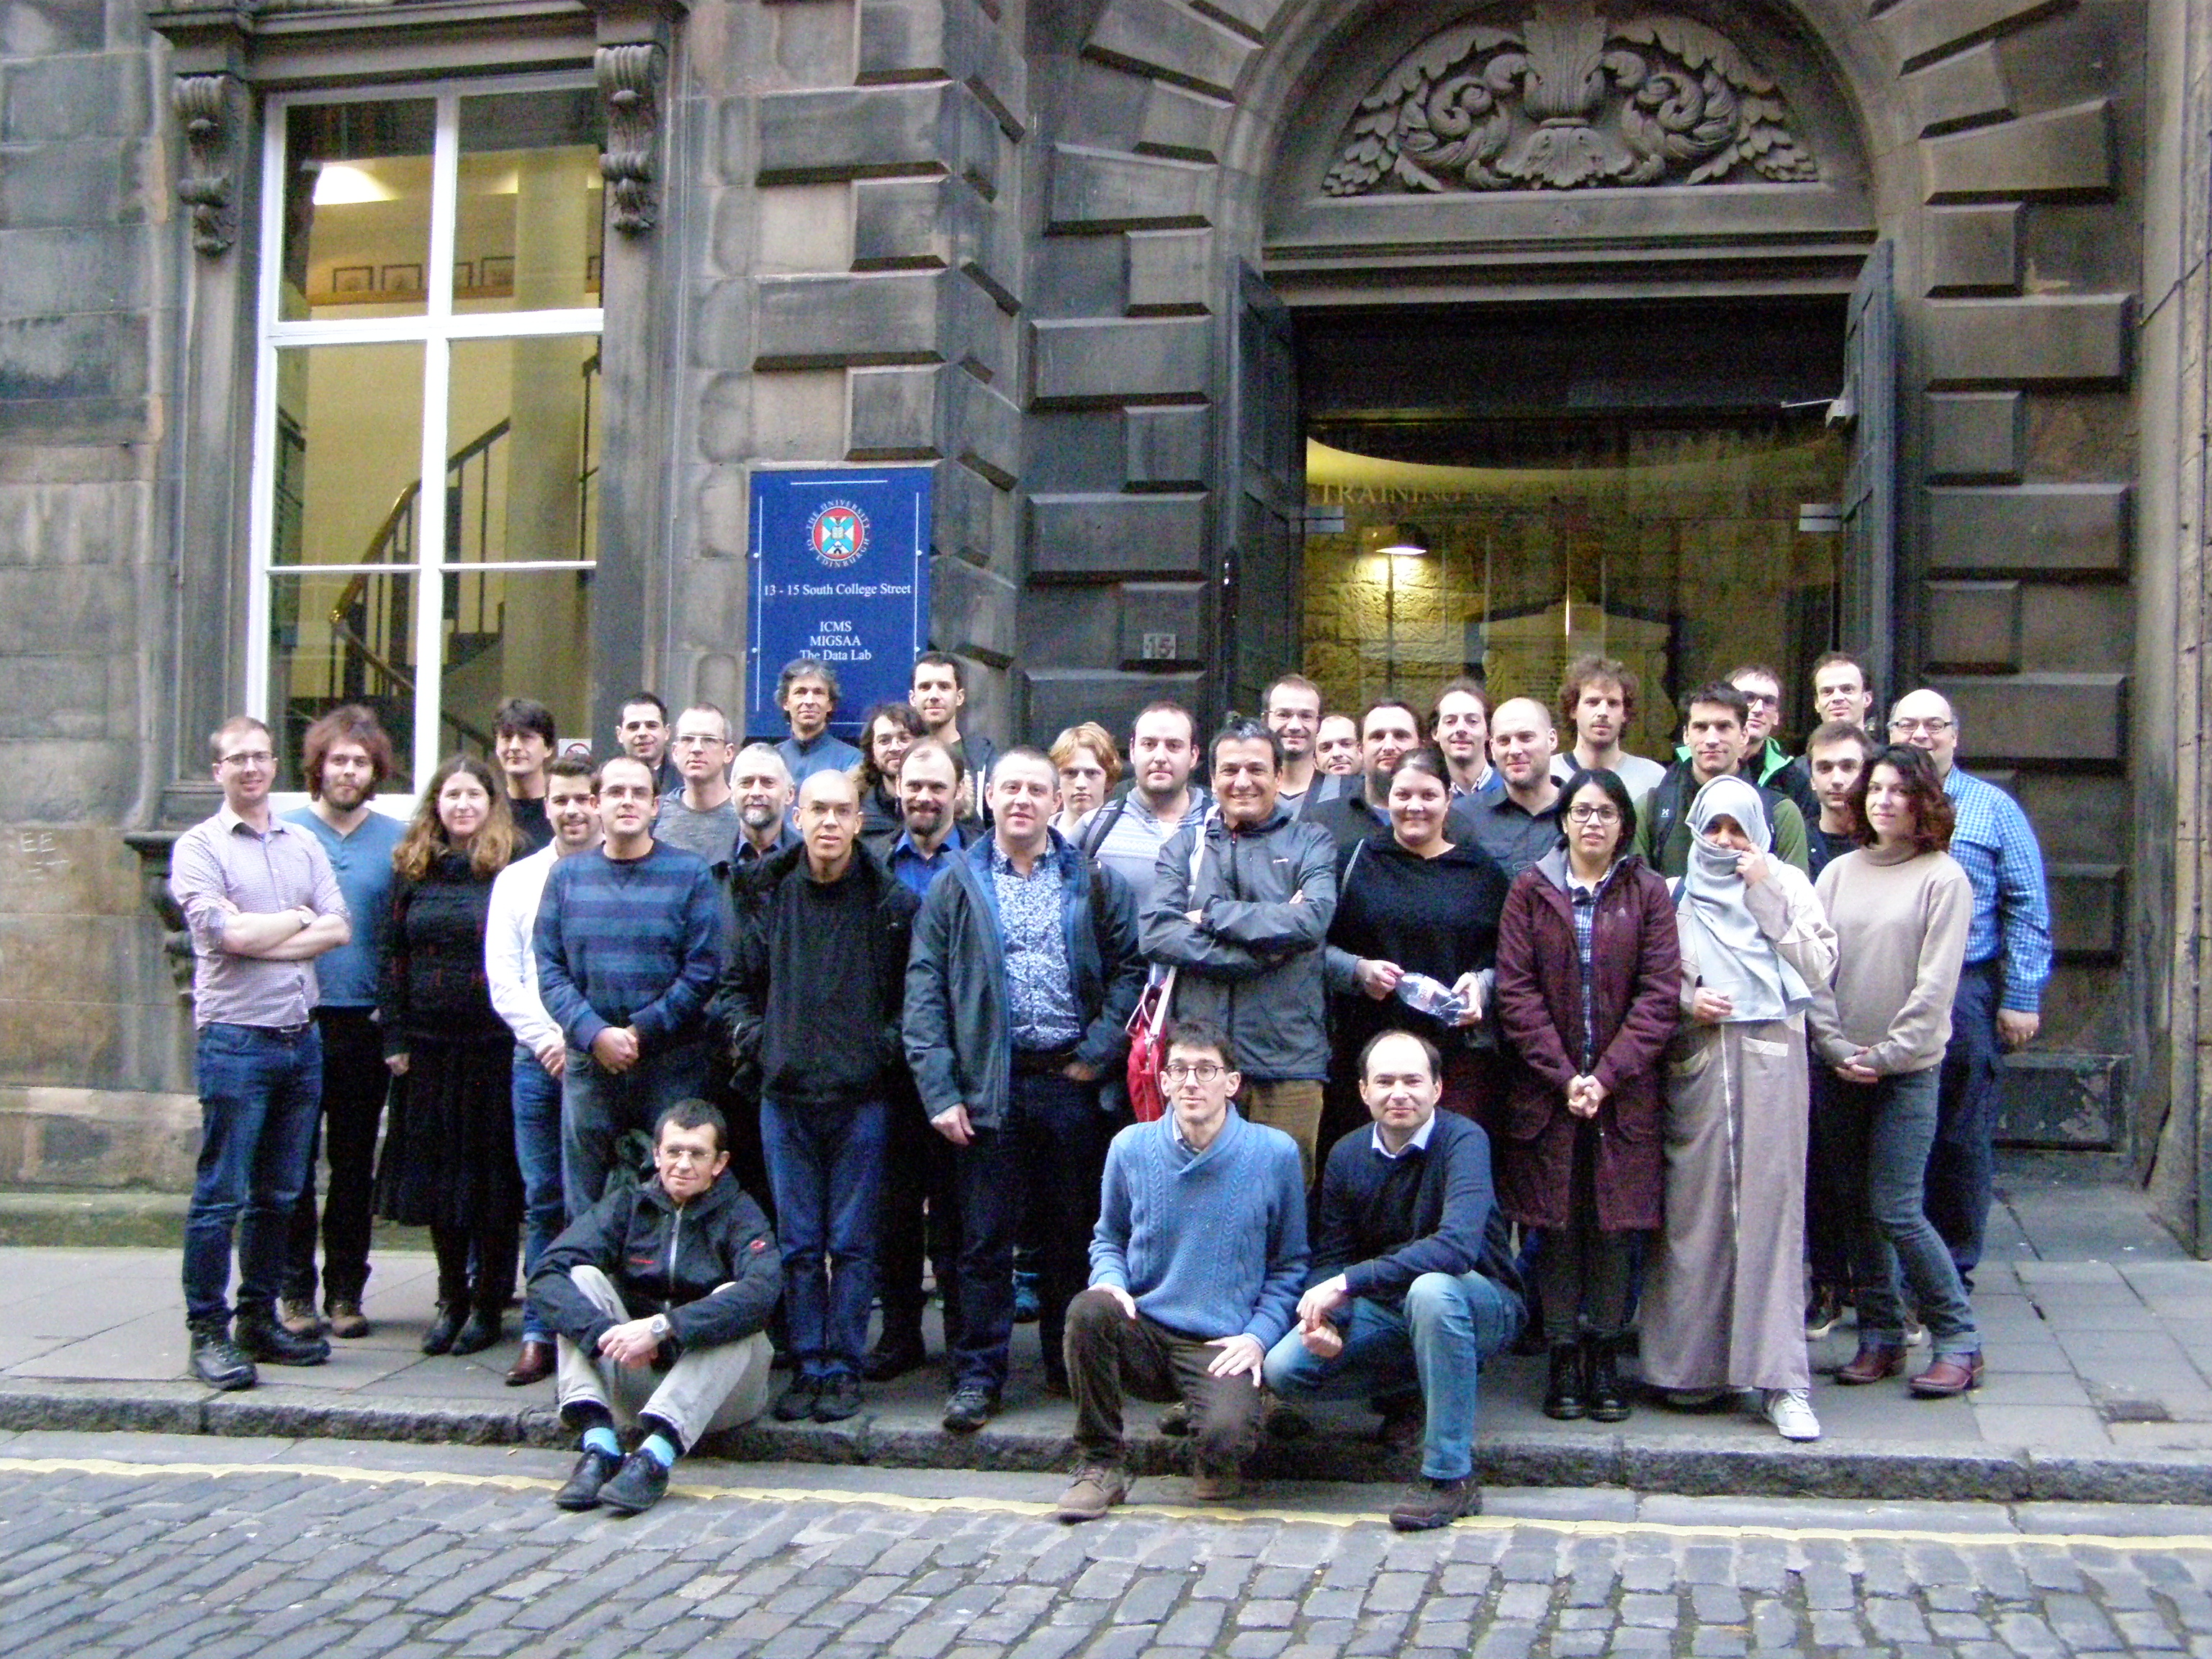
\includegraphics[scale=.14]{ICMS_Jan2017.jpg}
\caption*{Participants of the workshop ``Computational Mathematics with Jupyter''}
\end{figure}

\end{event}

\begin{event}{IOP Magnetism 2017 - Computational micromagnetics with JOOMMF workshop}{IOP2017}{University of York, UK, 04 April 2017}{XFEL}{30}{3}{http://magnetism2017.iopconfs.org/OOMMF}

\textbf{Main goals.} We introduced the basics of micromagnetics as well as taught the participants how to run OOMMF simulations using our Python interface - JOOMMF.

\textbf{ODK implication.} JOOMMF was developed as a part of the ODK project and three participants from the ODK were present to deliver the workshop (Hans Fangohr, Marijan Beg, and Ryan A. Pepper). The workshop was co-funded by the conference organisers and the EPSRC CCP Computational Magnetism Network (EP/M022668/1) grant. No costs of the workshop were paid from the ODK funds.

\textbf{Event summary.} In this workshop we provided a brief introduction to computational micromagnetics, Python, and the Jupyter notebook. We taught participants to use our Python interface to drive OOMMF micromagnetic simulation by guiding them through tutorials. At the beginning of the workshop, we provided a lecture style introduction, which was followed by practical exercises where attendees had an opportunity to carry out small micromagnetic calculations, modify given examples and ask more specific questions. This workshop was held together with Michael Donahue, NIST - one of the main developers of the OOMMF package.

\textbf{Demographic.} We had about 30 participants during the workshop, but due to the data protection regulations, the organisers did not allow us to have demographics information. During the workshop, 19 participants gave us their details with demographics: 13 males and 6 females.

\textbf{Results and impact.} During the workshop we received the feedback from the participants about our Python interface to OOMMF as well as gained experience which helped us to structure future workshops.

\end{event}


\begin{event}{Intermag 2017 - Computational micromagnetics with JOOMMF workshop}{Intermag2017}{Dublin, Ireland, 24 April 2017}{XFEL}{57}{2}{}

\textbf{Main goals.} We introduced the basics of computational micromagnetics as well as taught the participants how to run JOOMMF simulations.

\textbf{ODK implication.} JOOMMF was developed as a part of the ODK project and two participants from the ODK project were present to deliver the workshop (Marijan Beg, and Ryan A. Pepper). The workshop was co-funded by the conference organisers and the EPSRC CCP Computational Magnetism Network (EP/M022668/1) grant. No costs of the workshop were paid from the ODK funds.

\textbf{Event summary.} In this workshop we provided a brief introduction to computational micromagnetics. We introduced and taught the use of a Python interface to drive the OOMMF simulation package. At the beginning of the workshop, we provided a lecture style introduction, which was followed by practical exercises where attendees had an opportunity to carry out small micromagnetic calculations, modify given examples and ask more specific questions. Several days after the main event, we held a follow up session, where we were able to talk to participants about their specific needs, get requests for features, and get general feedback.

\textbf{Demographic.} We had 57 participants, but the organizers did not allow us to have their personal details.

\textbf{Results and impact.} During the workshop we received the feedback from the participants about our Python interface to OOMMF as well as gained experience which helped us to structure future workshops.

\begin{figure}[ht]
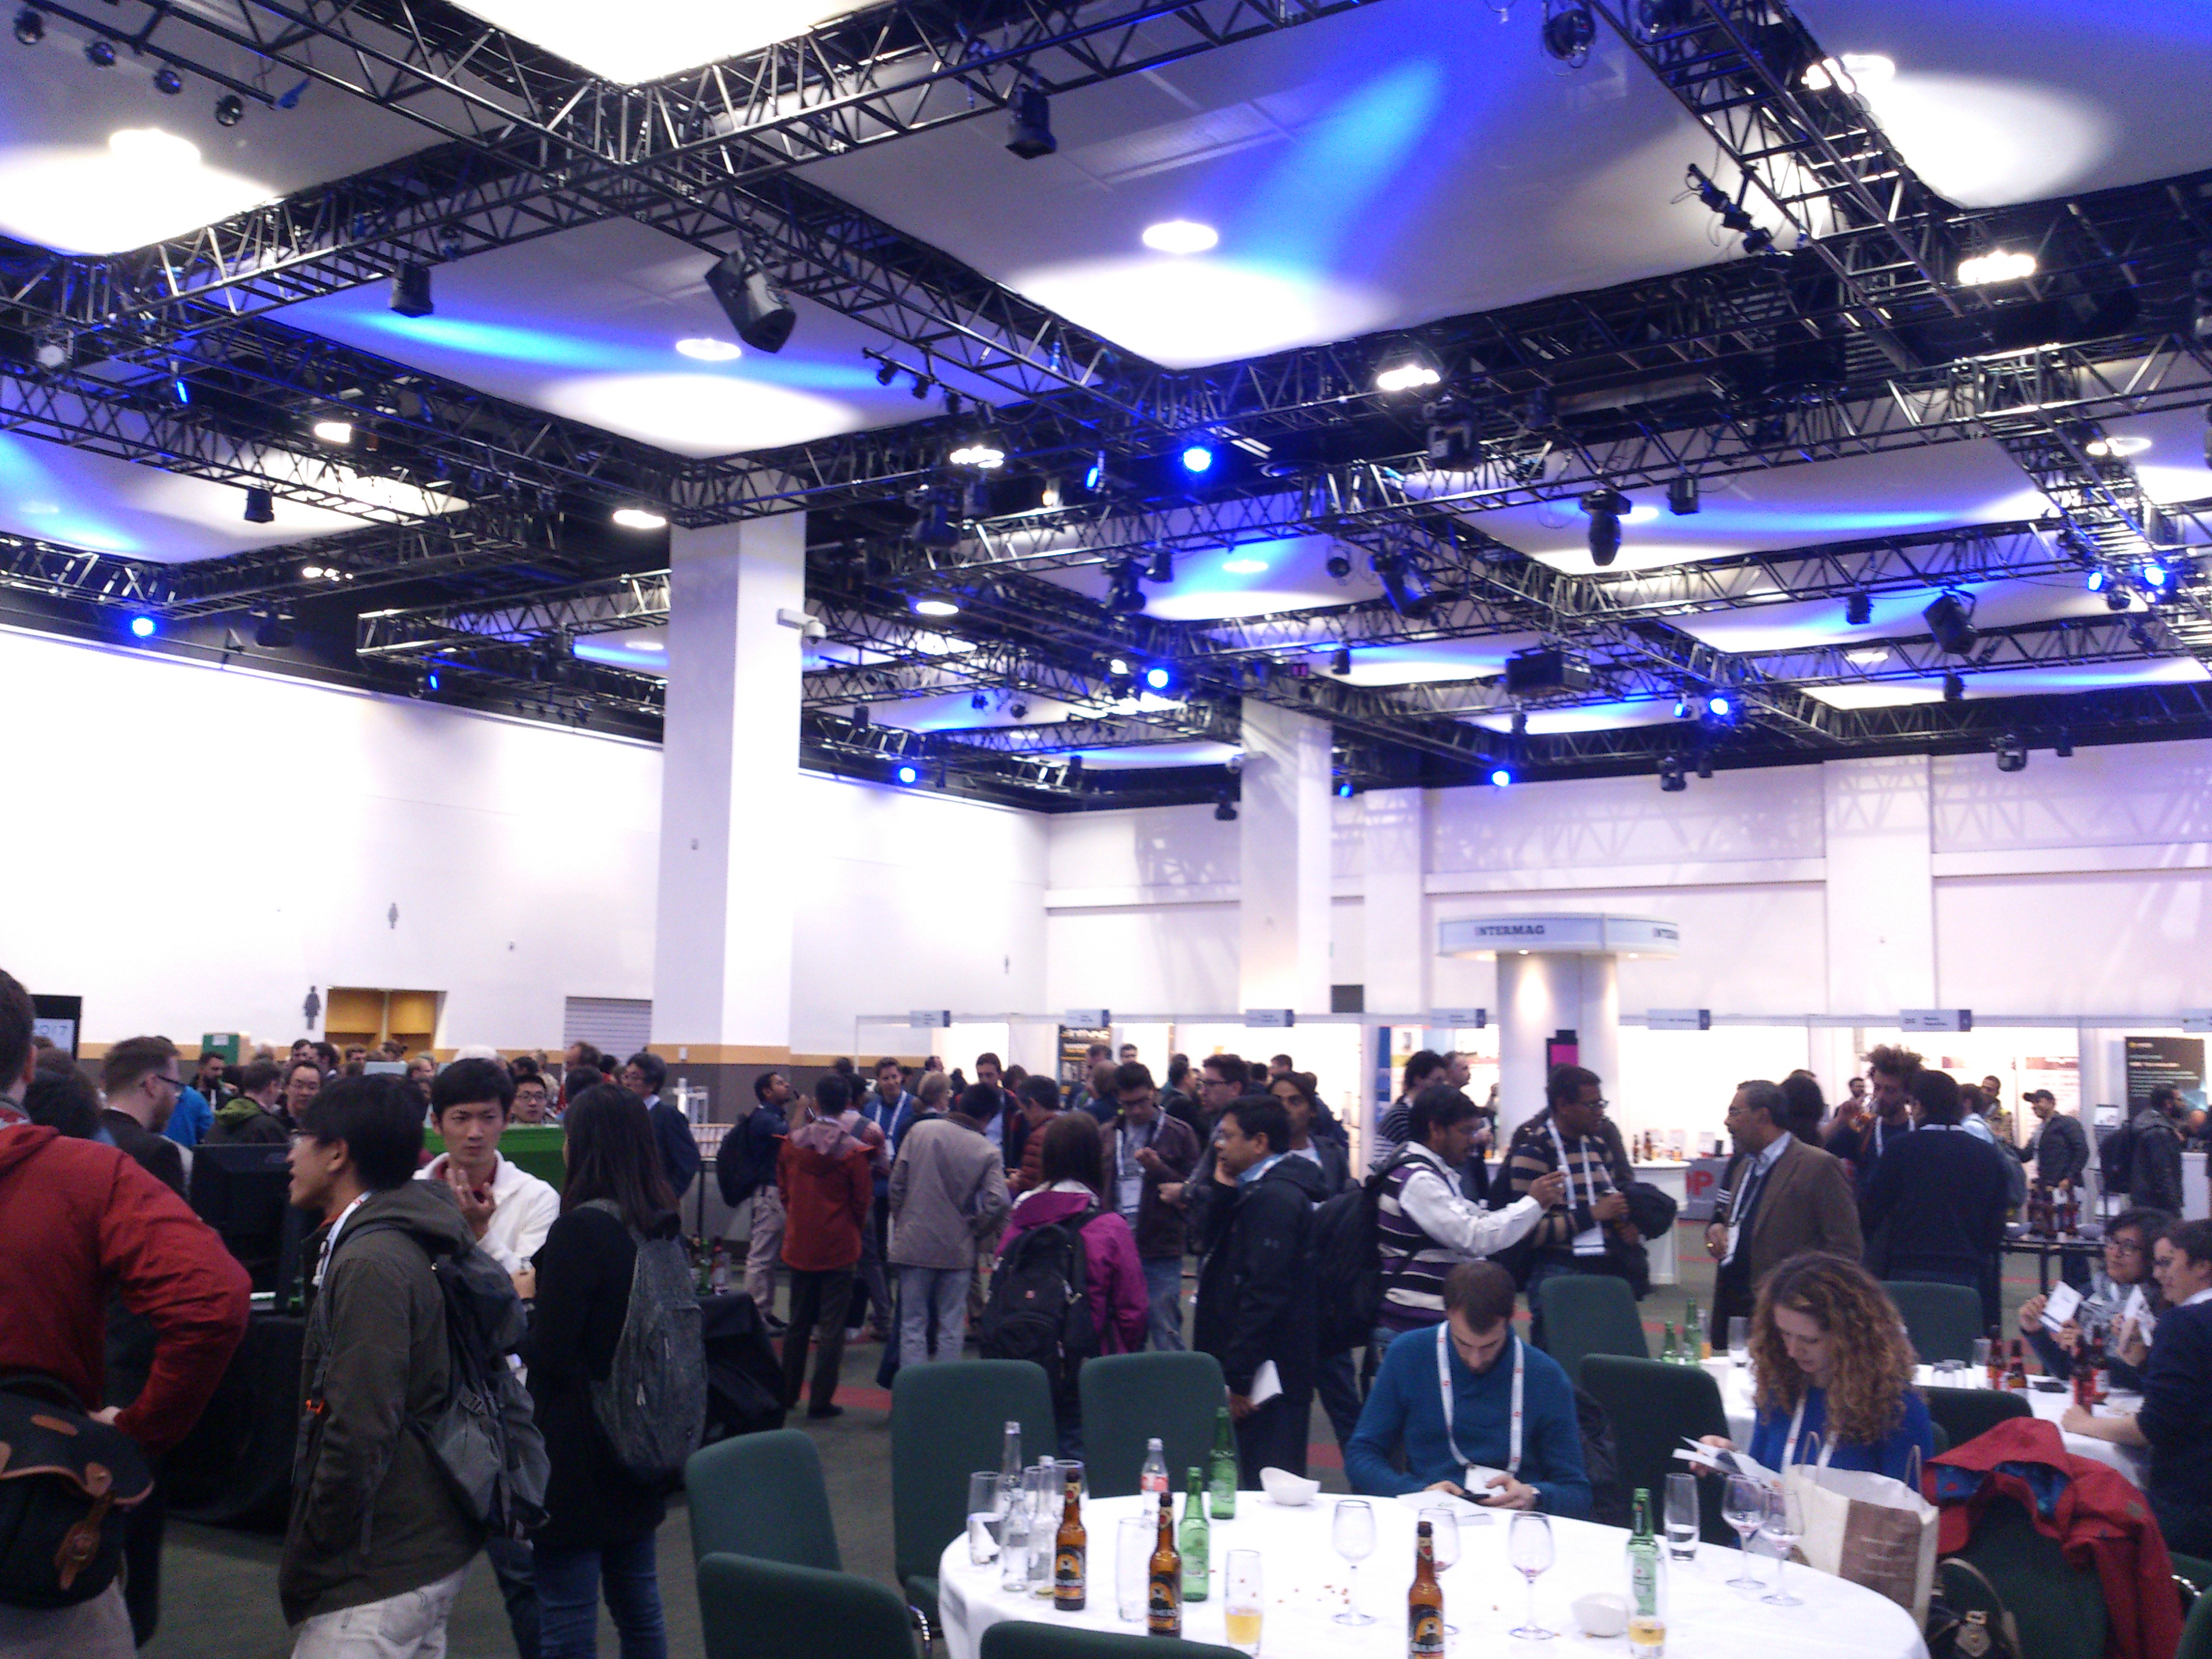
\includegraphics[scale=.1]{IntermagPhoto1.jpg}
\caption*{Intermag2017 conference in Dublin, Ireland.}
\end{figure}

\begin{figure}[ht]
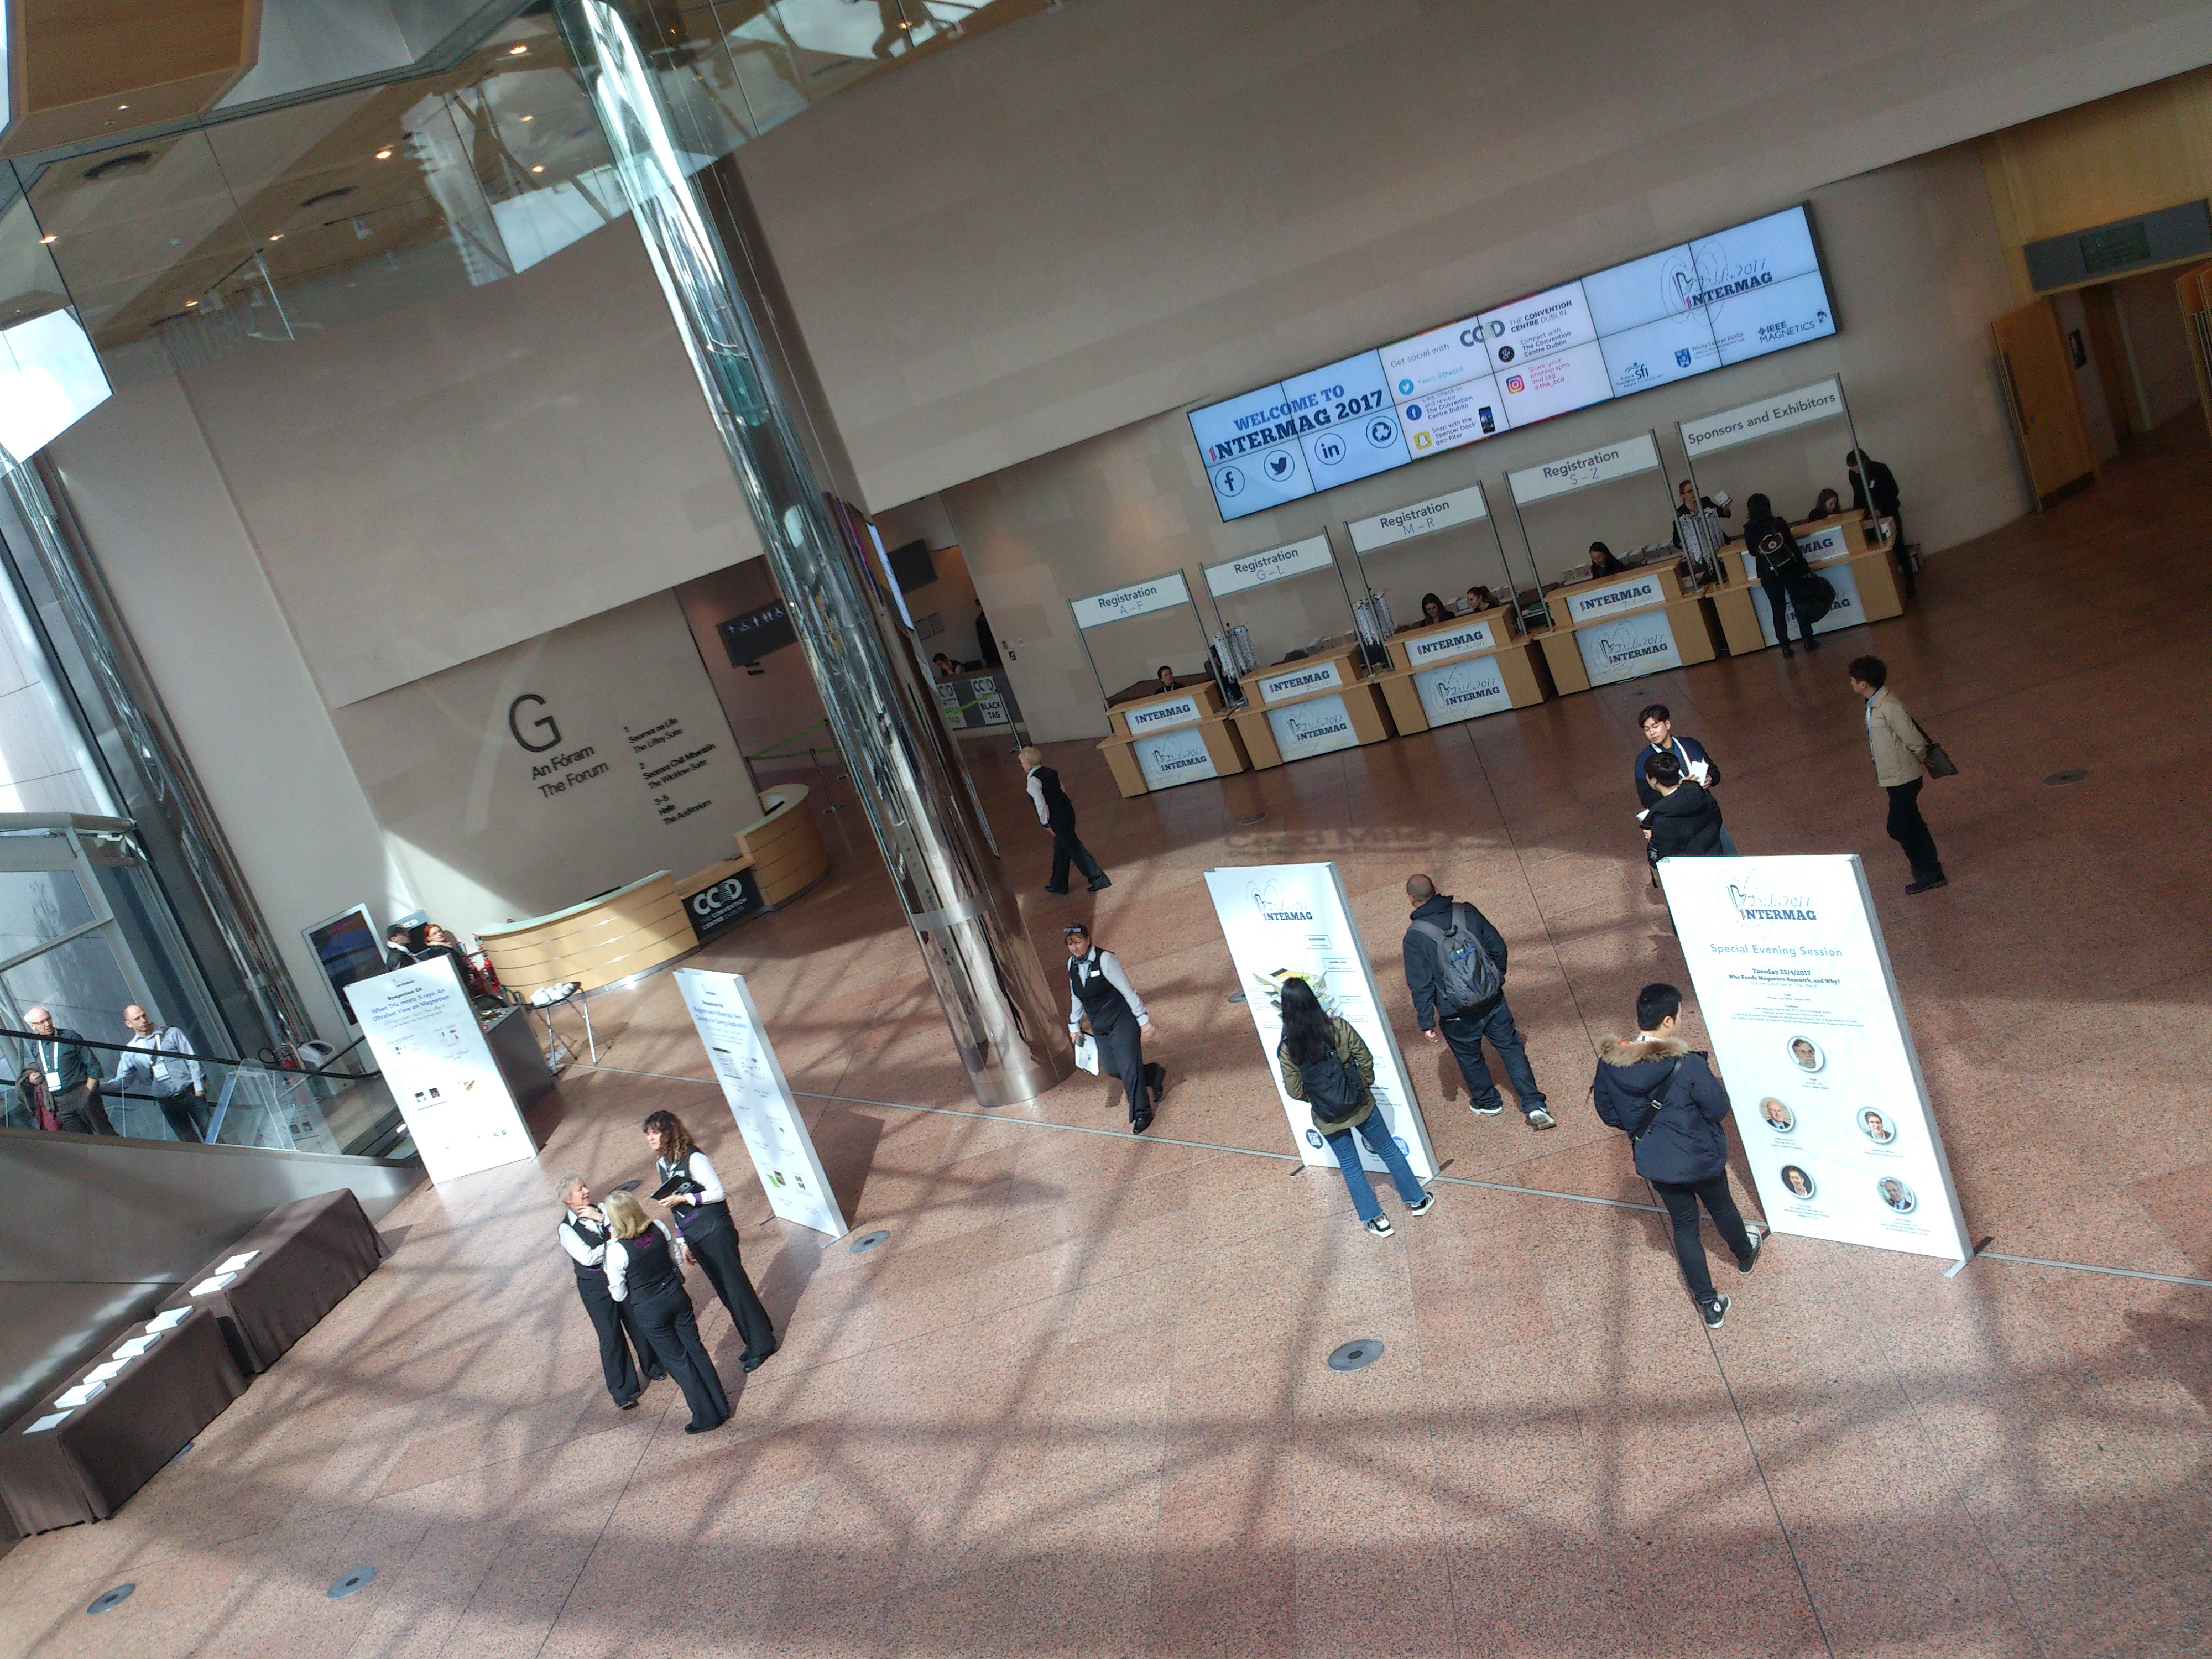
\includegraphics[scale=.1]{IntermagPhoto2.jpg}
\caption*{Intermag2017 conference in Dublin, Ireland.}
\end{figure}

\end{event}


\begin{event}{MMM 2017 - JOOMMF drop-in sessions}{MMM2017}{Pittsburgh, PA, USA 06-10 November 2017}{XFEL}{5}{1}{}

\textbf{Main goals.} In two sessions during the conference, users had a chance to talk to us, give us feedback, and request features.

\textbf{ODK implication.} JOOMMF was developed as a part of the ODK project and one participant from the ODK was present to deliver the workshop (Marijan Beg). The workshop was fully funded by the ODK and total costs were 2048.67 euros.

\textbf{Event summary.} In two drop-in sessions, we helped users with installation, looked at their simulation requirements, and received some feedback and feature requests.

\textbf{Results and impact.} During the workshop we received the feedback from the participants about our Python interface to OOMMF.

\end{event}


\begin{event}{Bioinformatics Awareness Days}{SHF_BAD}{University of Sheffield, November 2017 }{USH}{30}{2}{https://bitsandchips.me/BAD_days/}

\textbf{Main goals.} The ecosystem of tools supported by the OpenDreamKit project are suitable for a wide range of scientific disciplines. The development of this workshop, in collaboration with a bioinformatics practitioner, was an experiment in how to apply ODK supported technologies to the field of Bioinformatics.

\textbf{ODK implication.} Workshop materials were developed by Tania Allard in collaboration with Statistician and Bioinformatics researcher, Dr Luisa Cutillo.  The materials were released online at \url{https://github.com/trallard/BAD_days}. The workshop was delivered by Dr Cutillo with support from Tania Allard.

\textbf{Event summary.} A group of researchers based within the Sheffield Institute for Translational Neuroscience (SITRAN, \url{http://sitran.org/}) were taught about Bioinformatics workflows using Jupyter notebooks with computation provided by the free Micosost Azure Notebook service.

\textbf{Results and impact.} The event demonstrated that ODK supported technologies could be applied to the field of Bioinformatics and led to a new collaboration between Dr Cutillo and ODK member Mike Croucher.

Following the success of this workshop, Dr Cutillo independently taught an introductory workshop on statistics using Jupyter notebooks on Azure at Parthenope University of Naples (Materials at \url{https://github.com/luisacutillo78/RbasicStats})

Dr Cutillo has since moved to University of Leeds where she will be teaching statistics to 200+ undergraduates. She plans to use ODK developed technologies in collaboration with the Research Software Engineering group at Leeds.

The event required the development of a website that was linked to the Jupyter notebooks (\url{https://bitsandchips.me/BAD_days/}). The website caught the attention of Eleni Vasilaki, Head of Machine Learning at University of Sheffield who wanted to do something similar for her course on Adaptive Intelligence. We supported her in this endeavour and the result is at (\url{http://bitsandchips.me/COM3240_Adaptive_Intelligence/}).

In order to better support this, ODK member Tania Allard, developed a Jekyll template for use by academics and researchers using Jupyter notebooks for course materials and dissemination. Such a template allows the creation of Jupyter notebooks based websites using Jekyll, which is the default static website framework supported by GitHub. It also allows for easy display of notebooks connected to cloud computing resources such as Microsoft Azure Notebooks (D2.17, T2.6).

This led to the development of a Python package: nbjekyll (\url{https://github.com/trallard/nbjekyll}) that complements the Jekyll template. This package converts Jupyter notebooks into .md files that can be readily usable by Jekyll (this uses nbformat for the conversion). It also uses ODK-developed nbval to perform notebook validation and add custom headers indicating the last update date, version and test status of the notebook.

As well as being used internally at Sheffield, The nbjekyll package received some attention on twitter \url{https://twitter.com/jdblischak/status/1009800776305332224} and \url{https://twitter.com/walkingrandomly/status/1009414151716909057} receiving a total of 42 retweets and 80 'likes'

\end{event}


\begin{event}{Advances in Magnetism 2018 - Computational micromagnetics with JOOMMF tutorial}{AIM2018}{La Thuile, Italy, 04-07 Fabruary 2018}{XFEL}{100}{1}{No url.}

\textbf{Main goals.} We gave a tutorial about computational micromagnetics and JOOMMF to all conference participants.

\textbf{ODK implication.} JOOMMF was developed as a part of the ODK project and one participant from the ODK was present to deliver the tutorial (Marijan Beg). The tutorial was fully funded from the ODK funds and the total costs were 1207.73 euros.

\textbf{Event summary.} This tutorial was in the official part of the conference programme available to all atendees. We had about 100 participants and we introduced to them the basics of computational micromagnetics as well as gave them an introduction to JOOMMF. At the end, we answered any specific question attendees had.

\textbf{Demographic.} We had around 100 participants, but the organisers did not allow us to have their personal details due to the data protection.

\textbf{Results and impact.} We informed the community of potential users about the benefits of JOOMMF and provided to them enough information if they want to start using it.

\end{event}


\begin{event}{Introduction to HPC using the Jupyter notebook}{SHF_HPC}{University of Sheffield, 12th of April 2018}{USH}{15}{2}{https://github.com/RSE-Sheffield/hi-perf-ipynb}

\textbf{Main goals.} Previous ODK work provided us with Sun Grid Engine Support for Project Jupyter Hub (Deliverable 5.3) which gave users of High Performance Computing systems, such as the one at University of Sheffield, access to powerful supercomputer hardware via the notebook. This workshop acted to disseminate this work, encourage more people to use HPC via the newly developed interface and teach the basics of parallelisaton in Python.

\textbf{ODK implication.} Workshop materials were developed by Will Furnass (USH) and released online at \url{https://github.com/RSE-Sheffield/hi-perf-ipynb}. The workshop was delivered by Will Furnass and Mike Croucher at University of Sheffield.

\textbf{Event summary.} A group of researchers from a cross-section of subjects were taught the basics of parallelization and HPC using ODK developed technologies and tutorials. The event was publicized on twitter which lead to follow up queries about the underlying technology. 

\textbf{Results and impact.} The event established that the technology is scalable enough to be used in production for a typical class size at HPC training events. The ODK developed technology is now a permanent part of the HPC service at University of Sheffield with ongoing work continually released at \url{https://github.com/RSE-Sheffield/jupyterhub-gridengine-sharc}

\end{event}


\begin{event}{Atelier PARI/GP 2018b}{AtelierPARI2018b}{Roma (IT),
2018-04-16 to 2018-04-17}{UB}{36}{6}{http://pari.math.u-bordeaux.fr/Events/PARI2018b/}

\textbf{Main goals.}

This was a teaching and dissemination meeting, by invitation from the Roman
  Number Theory Association as a satellite event for their 4th
  mini-symposium.

\textbf{ODK implication.} 
%Describe how ODK was involved and give a rough estimation of cost for ODK

\ODK participants: B. Allombert and A. Page from Bordeaux.

\ODK funded travel and accomodation costs for the two instructors for about
  3k\euro. The ALGANT consortium, LIA LYSM (CNRS) and University Roma Tre
  co-funded the event.

\textbf{Event summary.} 
%Give a summary of your event

This Atelier PARI/GP took place in Roma (Italy) from april 16th to
17rd, it was followed by a 3-day international research conference on
  Number Theory. There were 30 participants for the Atelier.

The 2-day Atelier followed the same pattern as the preceding Oujda Atelier,
featuring a general introduction to PARI/GP and two 
  specialized courses (graduate level) in the mornings:
\begin{itemize}
\item Bill Allombert ``Elliptic curves over finite fields and number fields'',
\item Aurel Page ``Algebraic number theory''.
\end{itemize}
Afternoons were devoted to practice sessions.

Slides for all talks are available at
\url{http://pari.math.u-bordeaux.fr/Events/PARI2018b/}

\textbf{Results and impact.} 
% What did you achieve with this event? (If ever it impacted 
% other ODK tasks and deliverables, mention it here)

This was a successful teaching and dissemination event.
\end{event}


\begin{event}{Atelier et \'Ecole MathExp 2018}{MathExp2018}{Saint-Flour (FR),
2018-05-21 to 2018-06-01}{UB}{36}{3}{https://mathexp2018.sciencesconf.org/}

\textbf{Main goals.}

The MathExp school and atelier organized in Saint Flour was a unique
opportunity for young mathematicians to learn about computer science
and the tools developed in the framework of \ODK. The event
was divided in two weeks. The first one focused on 4 courses and
introductory tutorials with SageMath and Jupyter. During the second
week the participants were asked to develop programs related to their
own research projects.

\textbf{ODK implication.} 
%Describe how ODK was involved and give a rough estimation of cost for ODK

\ODK organizer: V. Delecroix

\ODK provided the main funding source for the workshop (accommodation,
subsistence and some of the travel expenses) for about 40K\euro. There were
also inscription fees and the event was cofounded with the CNRS.

\textbf{Event summary.} 
%Give a summary of your event

The school and atelier MathExp took place in Saint-Flour (France)
from May 21st to June 1st.

There were 22 registered participants.

A typical day of the school consisted of 2 courses and tutorials
on computers. During the atelier, participants worked on their
own research projects asking for help when needed.

The School featured 4 courses on computer science topics directly
related to mathematical computations: probability (Ana Bušić (Paris, FR)),
linear programming (Xavier Goaoc (Marne-la-Vallée, FR)), formal computation
(Bruno Salvy (Lyon, FR)) and backtracking techniques (Michaël Rao (Lyon, FR)).

\textbf{Results and impact.} 
% What did you achieve with this event? (If ever it impacted 
% other ODK tasks and deliverables, mention it here)

We were delighted to achieve a gender equidistribution among the participants
(10 female and 12 males) which is not often in Mathematics and Computer
Science.

The school and workshop were very productive and beneficial to disseminate
the work achieved in the various work packages. In particular
all the work around SageMath and Jupyter.

\end{event}


\begin{event}{Web data in Python}{sheff_WebData}{Sheffield, 18th, 21st, 22nd and 23rd of June 2018}{USH}{40}{1}{https://github.com/trallard/WebData_Python}

\textbf{Main goals} Teach Social Scientists how to use Python and Jupyter notebooks to interact with online data sets.

\textbf{ODK implication.} ODK was involved in this work via ODK-funded team member Tania Allard.

\textbf{Event summary.}

Web data in Python for non computer scientists is a set of Jupyter notebooks and materials on how to use Python to collect, clean and analyse web data.

 It was developed in conjunction with Sheffield Research Methods Institute (An organisation created to promote innovation in research methods that can be applied to the social sciences to ultimately help solve the big challenges facing today’s society.)

In addition to developing and open sourcing the materials a workshop on the topic and using the materials was taught on May 18th, 21st, 22nd and 23rd along with other Software Carpentry workshops.

\textbf{Results and impact.} Materials are available online at \url{https://github.com/trallard/WebData_Python}

\end{event}


\begin{event}{2018 Leeds: Introduction to reproducible workflows in Python}{leeds_repro_python}{University of Leeds, June 14th 2018}{Leeds}{20}{1}{http://arc.leeds.ac.uk/training/spc-1-introduction-to-reproducible-workflows-in-python/}

\textbf{Main goals.} To introduce researchers at University of Leeds to good practice in reproducible research.

\textbf{ODK implication.} ODK member, Tania Allard, reused material developed by her for PyCon 2018 for this one day event.

\textbf{Event summary.} This is an introductory course to reproducible analysis workflows in Python. It is aimed at people with some experience in Python for data analysis or computational research (e.g. people already developing scripts or using Jupyter notebooks). By the end of the course the attendees will have learnt about best practices for reproducible scientific code development and should be able to implement these techniques to their day to day workflows.

Materials at https://github.com/trallard/ReproduciblePython

\textbf{Results and impact.} Around 20 researchers received training.

\end{event}


\begin{event}{ICM 2018 - Computational micromagnetics with JOOMMF workshop}{ICM2018}{San Francisco, CA, USA, 15-20 July 2018}{XFEL}{130}{2}{No url.}

\textbf{Main goals.} In this workshop we taught the participants to run micromagnetic simulations using JOOMMF.

\textbf{ODK implication.} JOOMMF was developed as a part of the ODK project and two participants from the ODK were present to deliver the workshop (Marijan Beg, and Ryan A. Pepper). The workshop was fully funded from the ODK project and the total costs were 7259.58 euros.

\textbf{Event summary.} We started this 3.5 hours workshop by helping the participants to install all required software on their laptops. After that we introduced some physics basics of micromagnetics as well as theoretically explained how does a micromagnetic simulation work. After that we went through the tutorials and explained all individual commands of JOOMMF required for participants to complete the exercises. Finally, participants were working on an exercise and managed to reproduce the results from already published work. We had a lot of opportunity to talk to the existing and potential users and get feedback from them.

\textbf{Demographic.} We had around 150 participants, but due to the data protection we could not obtain any demographics data from them.

\textbf{Results and impact.} During the workshop we received the feedback from the participants about our Python interface to OOMMF as well as gained experience which helped us to structure future workshops.

\begin{figure}[ht]
\include{ICMPhoto1.jpg}
\caption*{JOOMMF workshop at ICM2018 conference in San Francisco, CA, USA}
\end{figure}

\begin{figure}[ht]
\include{ICMPhoto2.jpg}
\caption*{JOOMMF workshop at ICM2018 conference in San Francisco, CA, USA}
\end{figure}

\begin{figure}[ht]
\include{ICMPhoto3.jpg}
\caption*{JOOMMF workshop at ICM2018 conference in San Francisco, CA, USA}
\end{figure}

\end{event}


\begin{event}{GAP Tutorial at the 20th Postrgaduate Group Theory Conference}{PGTC2018}{St Andrews, Jul. 16 -- 20, 2018}{SA}{21}{1}{https://www.codima.ac.uk/pgtc2018/}

\textbf{Main goals.} The Postrgaduate Group Theory Conference (PGTC) is an annual meeting of
young researchers in group theory. The GAP Tutorial was organised as an optional satellite event.

\textbf{\ODK implication.} Although \ODK was not formally involved in this event, it was
organised by Alexander Konovalov, and was used to promote the project and its outcomes.

\textbf{Event summary.} The GAP Tutorial was intended for beginners without requiring
any prior knowledge of the GAP system. The first part on Monday July 16th covered
the Software Carpentry lesson ``Programming with GAP'' and was delivered in the live
coding style. The second part on Friday July 18th included a talk on debugging and
profiling in GAP by Christopher Jefferson (St Andrews) and a talk
``Using GAP Effectively: Some Tips and Pitfalls'' by Alexander Konovalov. The latter
included the demonstration of the GAP Jupyter interface as included in the GAP 4.9.2
release (June 2018). Using Jupyter notebooks for this talk contained in the repository
at \url{https://github.com/alex-konovalov/gap-teaching}, attendees were able to launch
them on Binder and try to work with GAP in Jupyter themselves. Several participants
received help with installing the latest release of GAP and configuring its Jupyter
kernel after the tutorial and left the event with fully usable working environment.

\end{event}


\subsection{Organization of Sage Days in established mathematical communities}

One goal of \ODK is to support local communities of researchers
and developers who contribute to the open-source software related to
the project. For \Sage, this means supporting the organization of Sage-Days
workshops that arise from within all the different mathematical communities. The main 
goal of these workshops is mostly to improve the Sage coverage of some mathematical
area. They also play a major role in training and communication. The
impact for \ODK can be summarized this way:

\begin{itemize}
\item \textbf{Making \ODK known to the end users}: by supporting Sage Days,
\ODK makes itself known to the Sage community and can
thus share the many developments of the project.

\item \textbf{Improving the overall quality of Sage}: by fostering researchers
in specific areas, Sage Days help bring interesting mathematics into
the software, which is beneficial for Sage and so \ODK.

\item \textbf{Training, bringing more user}: Sage Days are the perfect place
for new comers, especially students, to get their first experience with the software.

\item \textbf{Fostering a community}: Sage Days are helping making Sage a vibrant
community, which is vital for the success of \ODK.
\end{itemize}


\begin{event}{Sage Days 79}{SD79}{Jerusalem, Nov. 21 -- Nov. 24, 2016}{PS, UB}{46}{4}{https://wiki.sagemath.org/days79}

\textbf{Main goals.} This workshop was dedicated to the thematics ``geometric combinatorics and symbolic dynamics'' in \Sage. It was also a training program
for the local community in Israel with participants from the main universities (Herbrew University, Bar-Ilan University, Beer-Sheva, Ben-Gurion University, Tel-Aviv University, University of Haifa, Weizmann Institute)

\textbf{ODK implication.} The workshop was mostly organized locally by Jean-Philippe Labbé and funded by the ERC Grant entitled ``Avenues in Probabilistic and Geometric Combinatorics''. ODK was supporting the event by...

\textbf{Event summary.} The event started by introduction talks and tutorials as well as installation sessions about \Sage so that new comers could be initiated and guided. The rest of the week featured many specific tutorials about some mathematics features related to the thematic of the workshop. Lots of time was let open for coding and projects.

\textbf{Demographic.} 29 participants out of the 46 came from local universities in Israel. 

\textbf{Results and impact.} As the first Sage Days in Israel, the main objective of this meeting was to introduce the software to local participants. Around half of the participants were beginners, we made around 15 installations of \Sage on Windows, Mac and Linux. We allocated a lot of time for beginners to learn from tutorials but also directly from the more experienced users by personalized help. Having a flexible schedule allowed to have such help sessions.

Here is a summary of the accomplishments of the week:

\begin{itemize}
    \item    Worked was carried out on 47 \Sage tickets: \url{https://trac.sagemath.org/query?keywords=~days79}
    \item    Around 15 installations on Windows, Mac and Linux.
    \item    Creation of a sample \Sage package to document the process.
    \item    Around 10 participants got to know Sage better doing tutorials
    \item    Experienced Sage users answered tons of questions surrounding usage of Sage
    \item    We got 5-6 more experienced users to contribute to Sage by reviewing, reporting, writing tickets
    \item    Many discussions and healthy debates about view, plot, show and polytope in Sage
    \item    Some projects and discussions will be continued through future collaborations and meetings in 2017 
\end{itemize}


\end{event}

\begin{event}{Sage Days 84}{SageDays84}{Olot (ES),
2017-02-27 to 2018-03-10}{UB}{12}{2}{https://wiki.sagemath.org/days84}

\textbf{Main goals.}
The main goal of the Sage Days 84 were to
gather researcher specialists in polyhedral computations and advanced
SageMath developers.

\textbf{ODK implication.} 
%Describe how ODK was involved and give a rough estimation of cost for ODK

\ODK organizer: V. Delecroix.

\ODK participants: V. Klein

\ODK provided the funding source for the workshop (accommodation,
subsistence and travel expenses) for about 20k\euro.

\textbf{Event summary.} 
%Give a summary of your event

The Sage Days 84 took place in Olot (Spain) from february 2nd to
march 10th. It was focused on polyhedral computations.

There were 12 registered participants. A typical day of the workshop
consisted in talks and hacking session.

\textbf{Results and impact.} 
% What did you achieve with this event? (If ever it impacted 
% other ODK tasks and deliverables, mention it here)
This was a development workshop dedicated to researcher polyhedral
computations. We obtain interesting feedback especialy from
the polymake developers Julian Pfeifle and Andreas Paffenholz. One
of the achievement was the integration in SageMath of an interface
to polymake
(see \url{https://trac.sagemath.org/ticket/22452}).
\end{event}


\begin{event}{Sage/GAP Days 86: Algebra and Words in Combinatorics }{sd86}{Montréal (Canada) 2017-04-17 to 21}{PS}{31}{2}{https://wiki.sagemath.org/days86}

  \textbf{Main goals.} This training workshop was organized at the
  occasion of a four month CRM thematic semester
  [Algebra and words in combinatorics(http://www.crm.umontreal.ca/Combinatorics2017/index.php/)
  at the [Laboratoire de combinatoire et d'informatique mathématique (LaCIM)](http://lacim.uqam.ca/en/) of
  [Université du Québec à Montréal](http://www.uqam.ca/).

  Taking advantage of the participation of Nicolas M. Thiéry to the
  thematic semester (as member of the scientific committee), this
  workshop was followed by a
  \href{https://wiki.sagemath.org/Montreal}{weekly half-day meeting}
  around computational tools for combinatorics until July 2017, and
  \href{https://more-sagemath-tutorials.readthedocs.io/en/latest/2017-05-29-CRM/}{computational
    sessions} at the occasion of certain spring schools of the
  semester.

  \textbf{ODK implication.} The Sage Days was organized by Nicolas M.
  Thiéry (\ODK coordinator, Paris Sud) and Sébastien Labbé (since then
  \ODK participant at CNRS). \ODK funded some of the invited speakers
  (\approx 4k€). Later events were organized by Nicolas. Nicolas's
  participation to the semester (\approx 6k€) was funded by a
  combination of \ODK's direct and indirect costs.

  \textbf{Event summary.} An intensive week with many brainstorms and
  coding sprints + follow up meetings.

  \textbf{Demographic.} 31 participants (including 2 from \ODK), about
  half of which being female.

  \textbf{Results and impact.} Beside training many new \Sage users
  and developers, the workshop and followup events boosted an active
  local user group at LaCIM, including a new generation of graduate
  students and postdocs, but also François Bergeron, a prominent
  figure in experimental combinatorics who used the occasion to switch
  to \Sage. Discussions prompted the organization by this group of
  \Sage Days 95, a one week Women in \Sage workshop in July 2018,
  where \ODK member (Sheffield) and Research Software Engineer Tania
  Allard was invited as role model.

  Altogether
  \href{https://trac.sagemath.org/query?status=closed&status=needs_info&status=needs_review&status=needs_work&status=new&status=positive_review&keywords=~days86&col=id&col=summary&col=status&col=time&col=changetime&col=author&col=reviewer&order=status}{18
    \Sage tickets} were actively worked on during the week.
\end{event}


\begin{event}{Sage Days 93}{SageDays93}{Olot (ES),
2018-02-19 to 2018-03-04}{UB}{36}{1}{https://wiki.sagemath.org/days93}

\textbf{Main goals.}
The main goal of the Sage Days 93 were to
gather researcher specialists in Lie groups and advanced
SageMath and PARI/GP developers. The two goals were to implement
more Lie group theory in the softwares and conversely produce
experimental results for researchers.


\textbf{\ODK implication.}
%Describe how \ODK was involved and give a rough estimation of cost for \ODK

\ODK organizer: V. Delecroix.

\ODK provided the funding source for the workshop (accommodation,
subsistence and travel expenses) for about 20k\euro.

\textbf{Event summary.}
%Give a summary of your event

The Sage Days 93 took place in Olot (Spain) from february 19th to
march 4th. It was focused on the theory of Lie groups and their
subgroups.

There were 11 registered participants. A typical day of the workshop
consisted in talks and hacking session.

\textbf{Results and impact.}
% What did you achieve with this event? (If ever it impacted
% other \ODK tasks and deliverables, mention it here)
This was a development workshop dedicated to researcher in Lie groups
and their lattices. We obtain interesting feedback and developed
a lot of features related to Lie groups in SageMath and PARI/GP.
\end{event}


\begin{event}{Sage Days at Icerm}{SDIcerm}{ICERM Providence (United States), Jul. 23 -- 27, 2018}{PS}{78}{2}{https://icerm.brown.edu/topical_workshops/tw18-1-sage/}

\textbf{Main goals.} These Sage Days were focused on Combinatorics and Representation Theory. They were planned one week after the annual gathering of the algebraic combinatorics community at FPSAC 2018 (Hanover, New Hampshire).

\textbf{\ODK implication.} The event was not organized nor funded by \ODK. Nevertheless, it featured two talks by \ODK members (Nicolas Thiéry and Viviane Pons) and \ODK paid the travel expenses of some of the French participants.

\textbf{Event summary.} The event featured many presentations focusing on the link between \Sage development and research. It also allowed for some free coding time and discussions. Nicolas Thiéry and Viviane Pons both gave research presentations including some \Sage demo. It was an occasion to promote the \Sage docker and Jupyter live slides which is one of the use cases presented on \ODK website.

\textbf{Demographic.} Over 18 planed presentations, 9 were given by women.

\textbf{Results and impact.} This event was a good occasion for \ODK to connect the recent developments to the actual community and research. Beside \Sage development, many participants discovered docker during the event and showed lots of interest.

\end{event}




\subsection{Training activities in developing countries}

As open-source software developers, we wish our products
to be accessible to as many people as possible. Even though we offer
 a free access, there is still a technical gap in many 
developing countries that 
often prevents schools and researchers to benefit from our softwares.
This is why we believe the role of \ODK is to foster 
a wider community that does not leave a part of the world behind. In 
this section, we describe training activities that have been conducted 
through \ODK in this regard.

\begin{event}{Sage Days 89}{SageDays89}{University of science and technology Houari Boumediene, Algiers, Algeria, 2017-05-02 to 2017-05-07}{UB}{15}{1}{wiki.sagemath.org/days89}

\textbf{Main goals.} The first goal was to give some training on the SageMath system in order to implement new features  and/or to fix some bugs in SageMath. The second goal was to give some courses on Polya theory.

\textbf{ODK implication.} 
ODK financed the exhibitor's travel and accommodation.

\textbf{Event summary.} 
The Polya class was held in the morning from 9h to 13h every day for a week
for 10-15 students (Master 2 and PhD).
The course on Sage took place in the afternoon and evening from 15h to 21h-22h. (small committee of 4-5 participants).

\textbf{Results and impact.} Lessons on Polya and Sage system was correctly finished. The sage lesson was done by fixing a bug and producing the ticket 22979 on the trac server (\url{http://trac.sagemath.org/ticket/22979}).

\end{event}



\begin{event}{Atelier PARI/GP 2017c}{AtelierPARI2017c}{Oujda (MO),
2017-11-22 to 2017-11-23}{UB}{36}{6}{http://pari.math.u-bordeaux.fr/Events/PARI2017c/}

\textbf{Main goals.}

This was a teaching and dissemination meeting, by invitation from the math
institute in Oujda as a satellite event for their ``Journ\'ees Alg\`ebre,
  Th\'eorie des Nombres et Application''.

\textbf{ODK implication.} 
%Describe how ODK was involved and give a rough estimation of cost for ODK

\ODK participants: B. Allombert and A. Page from Bordeaux.

\ODK funded travel costs for the two instructors for about 1k\euro. The
  organizing Oujda institute of mathematics co-funded the event, paying for
  all local expenses.

\textbf{Event summary.} 
%Give a summary of your event

This Atelier PARI/GP took place in Oujda (Morocco) from november 22nd to
23rd, it was followed by a 2-day Moroccan national research conference on
  Algebra, Number Theory and their Applications. There were 70 participants
  from all over Morocco (no registration fees).

The 2-day Atelier featured a general introduction to PARI/GP and two 
  specialized courses in the mornings (graduate level):
\begin{itemize}
\item Bill Allombert ``Cryptographie et courbes elliptiques'',
\item Aurel Page ``Th\'eorie alg\'ebrique des nombres''.
\end{itemize}
Afternoons were devoted to practice sessions. Bill Allombert also gave
  a research talk on ``Aspects combinatoires et algorithmiques des fonctions
  $L$ d'Artin'' in the ensuing conference.

Slides for all talks are available at
\url{http://pari.math.u-bordeaux.fr/Events/PARI2017c/}

\textbf{Results and impact.} 
% What did you achieve with this event? (If ever it impacted 
% other ODK tasks and deliverables, mention it here)

This was the first purely instructional PARI/GP event, it allowed us to test
the format and teaching material, thereby paving the way for future such events.
\end{event}


\begin{event}{Software tools for mathematics 2018-01 Morelia}%
{STM_2018_01_Morelia}{Morelia, Mexico, 2018-01-22--2018-01-26}%
{PS}{50}{1}{http://matmor.unam.mx/software-tools-math/}

\textbf{Main goals.} The goal of the event was for mathematicians
to improve their coding skills and knowledge of mathematical software.

\textbf{ODK implication.} Samuel Lelièvre (ODK member from UPSud) was one of
the organisers. The OpenDreamKit funds at Paris-Sud were used to fund travel
and stays of speakers, and lunch and coffee breaks for all participants.
Centro de Ciencias Matemáticas (CCM), the mathematics department at
UNAM Morelia, co-funded the event, paying travel and accommodation for
some participants.

\textbf{Event summary.} The event consisted in a two-day Software Carpentry
workshop (teaching participants the Unix shell, version control with Git,
and programming with Python) followed by three days on mathematical software
with mini-courses on CoCalc, GAP, Jupyter, PARI/GP, SageMath, YAGS, as well
as talks on other mathematical software and databases, and on mathematical
research using software. A problem session allowed participants to submit
mathematical problems they cared about and thought software might help with,
several of which were solved in the following days by other participants.

\textbf{Demographic.} Over 140 people registered: 36\%\ bachelor students,
10\%\ master students, 14\%\ PhD students, 6\%\ postdocs, 20\%\ professors
and researchers, 10\%\ other. Since we could only welcome on the order of
50 participants, we focused on PhD students, postdocs, professors and
researchers.

\textbf{Results and impact.}

During the Software Carpentry workshop, Tania Hernandez taught the Unix shell,
Nelly Selem taught version control with Git, Leticia Vega taught programming
with Python. These courses were taught in Spanish, although using supporting
materials in English. This may have been the first time a Software Carpentry
workshop was taught entirely in Spanish. An effort is underway to translate
the Software Caprentry and Data Carpentry lesson plans to Spanish.

During the mathematical software part, Alexander Hulpke taught GAP, Samuel
Lelièvre taught CoCalc, Jupyter and SageMath, Miguel Pizaña taught YAGS
(a GAP package for working with graphs), Miguel Raggi presented Discreture
(a library for enumerating combinatorial objects), Emmanuel Royer taught
PARI/GP, Adrián Soto presented TeXmacs and gave a talk on Rauzy fractals,
Janoš Vidali presented DiscreteZOO, Rafael Villarroel presented Emacs,
Russ Woodroofe gave two talks ("The story of a calculation" and "The story
of a figure"), Katja Berčič gave a talk on "Databases of theorems", and
Uziel Silva gave a presentation of Macaulay2, Greuel and Reveal.js.

Many participants told the organisers, orally or by email, that this workshop
was transformative for them; often they felt they had passed some confidence
threshold: whereas before the conference they were interested in mathematical
software but unsure how to install and use them, they were now confident how
to do that, and felt they had the necessary resources to learn more.

One of the participants who is part of the board of the Mexican Math Society
initially intended to visit briefly to check out our workshop briefly, and
ended up staying the whole week, staying at the install party during the free
afternoon, and got convinced of the importance of having a software component
in future mathematics conferences in his area. As a result, David Sanders
gave a course on "numerical methods for dynamical systems", based on Julia,
at the next national dynamical systems conference in Mexico in June 2018.

Another of the organisers, Katja Berčič, a Slovenian post-doc currently in
Morelia, Mexico, liked the format of this workshop so much that a new workshop
on the same format is planned for September 2018 in Koper, Slovenia.

% \begin{figure}[ht]
% \caption*{A great picture of my wonderful event}
% Did you take pictures? Please share!
% \end{figure}

\end{event}

\begin{event}{6th Encuentro Colombiano de Combinatoria }{ECCO}{Barranquilla (Colombia), June 5 --- 16, 2018}{PS}{80}{1}{http://ecco2018.combinatoria.co/}

\textbf{Main goals.} ECCO (for \textit{Encuentro Colombiano de Combinatoria}) is a combinatorics research school organized every other year in Colombia. It gathered students from many countries (from both south-America and elsewhere) on advanced mathematics classes in an inclusive and welcoming environment. For the second time, it offered a \Sage class as well which goal is introduce \Sage to the students and help them develop their coding skills in relations to mathematics.

\textbf{ODK implication.} The \Sage class was given by Viviane Pons from ODK. Her travel costs were covered by ODK.

\textbf{Event summary.} Two afternoon sessions were organized (one for each week of the workshop). We had approximately 80 students on the first session and 40 on the second. Both sessions were organized in the computer room of the university so that all students would work whether they had material or not. Focus was given to introduction to \Sage in the context of combinatorics by offering many different tutorials and exercise worksheets for the students to choose from. We had created some specific worksheets in both English and Spanish directly related to the others courses of the conference so that the students could reproduce some of the results they had seen during classes and exercise sessions.

\textbf{Demographic.} We don't have access to the demographic information of the conference. Nevertheless we can say that most participants were students (from undergrad to PhD). Beside, this conference is in general very careful in creating a diverse and welcoming space.

\textbf{Results and impact.} This was the second time that we were at ECCO and we could see again that this was a great success. We had excellent feedbacks from both the students and the organizers. In 2016, the \Sage sessions were added late in the planning as extra sessions. In 2018, this is now an official \Sage course listed along the other mathematical classes of the conference. By being present twice in a row, we started a tradition of offering \Sage classes during this conference and this will be continued even after the end of ODK. For many students attending ECCO, the \Sage class is their first encounter with \Sage or even a mathematic software.

\begin{figure}[ht]
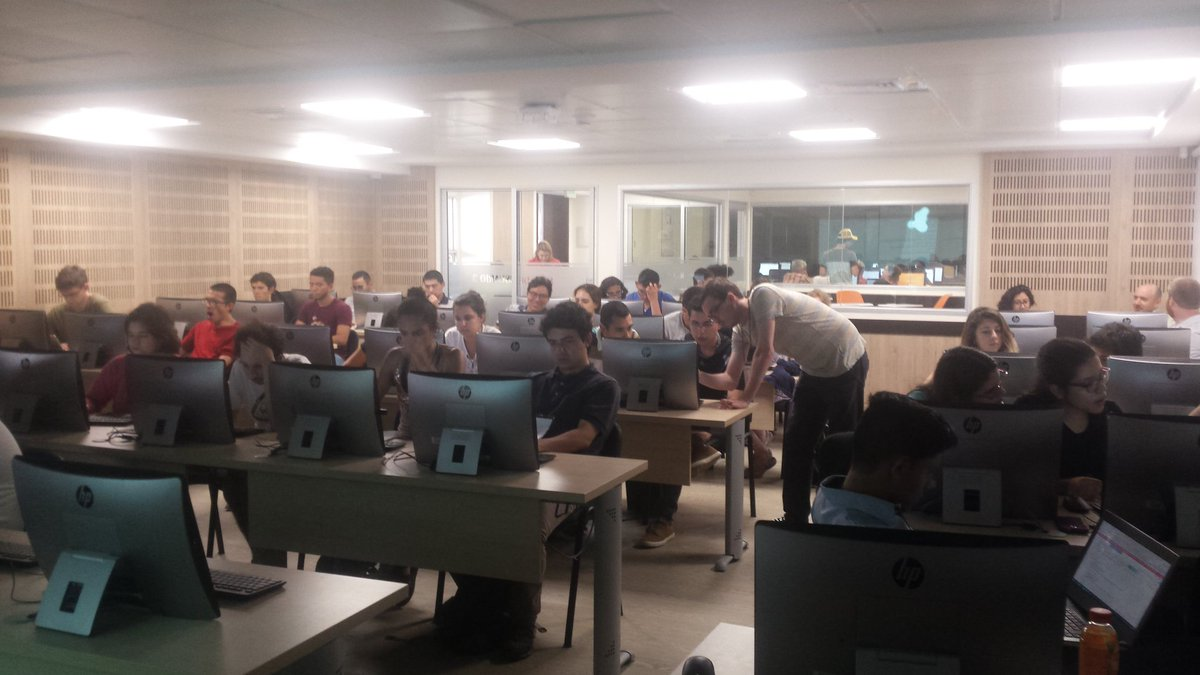
\includegraphics[scale=.2]{ECCO.jpg}
\caption*{Students working at ECCO}
\end{figure}



\end{event}

\subsection{Women in \ODK}

\ODK is aware of the gender gap that exists in science in general
and more specifically in software development. We have been organizing
events to support specifically women developers, engineers and scientists.

\begin{event}{Sage Days 82 : Women in Sage}{SD82}{Ris-Orangis (France), Jan. 9 -- Jan. 13, 2017}{PS}{20}{19}{https://wiki.sagemath.org/days82}

\textbf{Main goals.} The main goal of the event was to initiate more women to the software \Sage to reduce the gender gap in mathematics software
development. Each participant had to propose a mathematic development project to be carried out during the week.

\textbf{ODK implication.} The event was initiated by Viviane Pons from ODK and co-organized with Jennifer Balakrishnan (Boston University) and Jessica Striker (North Dakota State University). It was funded solely by ODK and cost around XXX in total, which covered: transportation for the organizers, lodging for the participants (rented house) and local food cost. 

\textbf{Event summary.} The opening event was a series of three lectures at Institut Henri-Poincaré on \Sage and research given by the three organizers. This was followed by a one-week workshop in a rented house in Ris-Orangis. There, we organized short talk sessions to get to know our respective research fields and expectations for the week. After that, we were able to split into small groups to work on many different projects: STL export, Krummer surfaces, Kuznyechik cipher, Motzkin words, Shioda invariants, and more. We also had presentations on ``How to contribute to Sage'' (with a crash course on git) and ``How to write a Sage package''. Every evening, we had a Status report session to share our progress with the group. We concluded the event with a joint coding afternoon in Paris with the PyLadies group.

\textbf{Demographic.} All participants were women coming from 7 different countries (France, US, Russia, Belgium, Greece, Austria, and Spain). About half of them could be considered Sage beginners. We had 7 PhD students, 4 postdoc or ATER, 8 \textit{Maîtresses de conférences} or Assistant professor and 1 Emeritus professor. 

\textbf{Results and impact.} A full report on the impact of this workshop can be read on our website \cite{17PonsSD82}. The main goal was to make the participants more confident into their programming skills and more prone to become Sage contributors and attend classical Sage Days. It was a big success in that regard. Indeed, before the conference, only 18\% of the participants had attended Sage Days more than once and 35\% had never heard of it. After, the conference, 100\% rated to 3 or more over 5 the chances that they would attend Sage Days event in the future. 94\% of the participant rated to 4 or more over 5 the impact of the workshop on their future career and 100\% rated the atmosphere of the conference 5 over 5. Besides, worked was done on 14 Sage tickets including 8 first contributions to Sage.

\begin{figure}[ht]
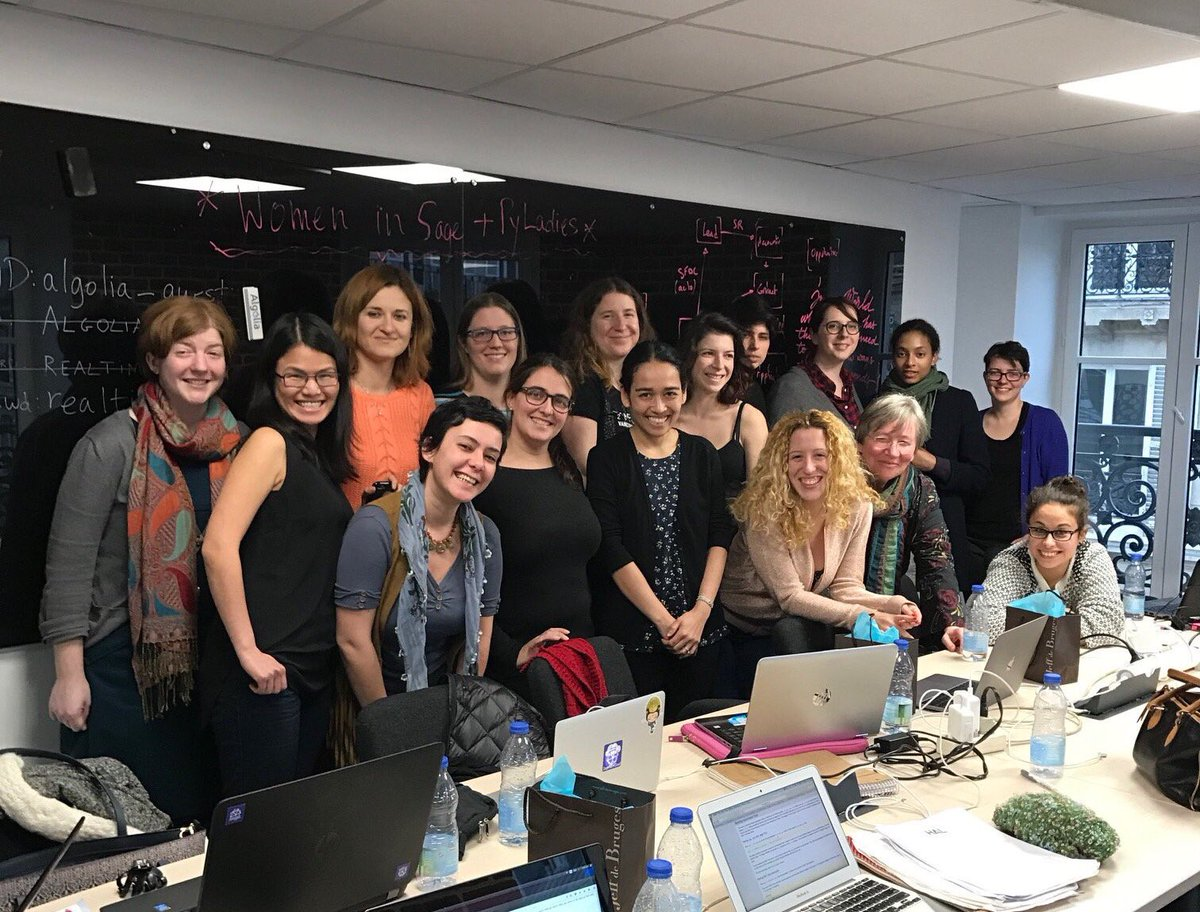
\includegraphics[scale=.2]{pyladies-WIS.jpg}
\caption*{The Women in Sage at the PyLadies coding afternoon}
\end{figure}



\end{event}

\begin{event}{Code First: Girls}{SHF_CFG}{University of Sheffield, 2017-2018 }{USH}{120}{1}{https://rse.shef.ac.uk/blog/codefirstgirls-meets-hacktoberfest/}

\textbf{Main goals.} Code First: Girls https://www.codefirstgirls.org.uk/ is an international organisation that works with companies and women to increase the numbers of women in technology.

\textbf{ODK implication.} ODK Sheffield team member, Tania Allard, worked with Code First:Girls chapters in Sheffield and Manchester over a 12 months period.

\textbf{Event summary.} Several events were run over a 12 month period which eventually provided training to over 130 women.  Tania developed materials on 'Advanced Python' using Jupyter Notebook which are now freely available at https://github.com/trallard/CodeFirst-Python_material

\textbf{Results and impact.} 130 women received training and new materials were developed for use in future Code First: Girls events.

\end{event}


\begin{event}{Diversity and Inclusion in Scientific Computing}{SHF_DISCU}{New York, 29th and 30th November 2018}{USH}{50}{1}{https://pydata.org/nyc2017/diversity-inclusion/disc-unconference-2017/}

\textbf{Main goals.} NumFOCUS's Diversity \& Inclusion in Scientific Computing (``DISC'') Program strives to help create a more diverse community through initiatives and programming devoted to increasing participation by and inclusion of underrepresented people.

\textbf{ODK implication.} ODK Sheffield member, Tania Allard was invited to participate in this 2 day event.

\textbf{Event summary.} At the inaugural Diversity and Inclusion in Scientific Computing (DISC) Unconference in November 2017 in New York, one of the topics that came up was organizing inclusive and diverse events and conferences. How to organize such an event? Is there a checklist? Is it hard? Participants decided to build on work begun by the NumFOCUS DISC Committee creating a cookbook for organizing inclusive and diverse events, with the aim of encouraging and supporting such events.

\textbf{Results and impact.} The output and its creation are described at \url{https://numfocus.org/blog/discover-cookbook}

\end{event}


\begin{event}{PyLadies Paris}{PyLadies}{Paris}{PS}{10}{1}{https://www.meetup.com/fr-FR/PyLadies-Paris/}

\textbf{Main goals.} The PyLadies organization is an international mentorship group with a focus on helping more women become active participants and leaders in the Python open-source community. PyLadies Paris is the local Paris chapter.

\textbf{ODK implication.} Viviane Pons from ODK has been the co-organizer of the PyLadies Paris events for the last two years. The Meetup group has 494 members and has had 57 events.

\textbf{Event summary.} Meetup include networking events for women coders such as ``Talking Bar'' and ``Coding Café''. They usually gather between 3 and 10 participants. Some events include presentations and / or tutorials on some specific subjects.

\textbf{Demographic.} These events are open to women who are interested in python. This include professional python developers, academics, scientist, students, and enthusiast learners.

\textbf{Results and impact.} We believe such events are very important to support women coders. They allow to build a strong professional network. It is also an occasion to discuss python practices and, in particlar, ODK developments in an informal and relaxed atmosphere.

\end{event}

\subsection{Organization of research workshopts}

\begin{event}{CICM2017 --- Conference on Intelligent Computer Mathematics}{CICM2017}{Edinburgh, UK, 17th-21st of July 2017}{FAU,JU}{45}{3}{https://cicm-conference.org/2017/cicm.php}

\textbf{Main goals.}
Digital and computational solutions are becoming the prevalent means for the generation, communication, processing, storage and curation of mathematical information.
Separate communities have developed to investigate and build computer based systems for computer algebra, automated deduction, and mathematical publishing as well as novel user interfaces.
While all of these systems excel in their own right, their integration can lead to synergies offering significant added value.
The Conference on Intelligent Computer Mathematics (CICM) offers a venue for discussing and developing solutions to the great challenges posed by the integration of these diverse areas. 

\textbf{ODK implication.}
Florian Rabe (JU) was track chair for Mathematical Knowledge Management.
One workshops was co-organized by Michael Kohlhase (FAU).
There were no costs to ODK other than travel costs for ODK members.

\textbf{Event summary.}
There were 17 formal paper presentations, 7 formal system presentations, 3 invited presentations, and 5 informal presentations.
Also, 2 workshops took place.

\textbf{Results and impact.}
The ODK participants presented the paper ``Classification of Alignments between Concepts of Formal Mathematical Systems'' that is integral to the MitM approach developed in ODK WP 6.
The authors included external collaborators in order to bundle system integration efforts.

Patrick Ion and Eric Weisstein presented ``The Special Function Concordance'', a development very closely related to the development of the MitM ontology of ODK WP 
\end{event}
 % 
\begin{event}{Modular Knowledge}{tetrapod2018}{Oxford, 2018-07-13}{FAU,PS}{20}{3}{https://kwarc.info/events/Tetrapod-2018/}

\textbf{Main goals.}
Expanding on the Tetrapod workshop at the conference on intelligent computer mathematics (CICM) 2016, this workshop brings together researchers from a diverse set of research areas in order to create a universal understanding of the challenges and solutions regarding highly structured knowledge bases.
Of particular interest are foundational principles such as theory graphs and colimits, interchange languages and module systems, languages and tools for representing, reasoning, computing, managing, and documenting modular knowledge bases.

\textbf{\ODK implication.}
This was co-organized by \ODK participants together with Jacques Carette, in order to connect with researchers in adjacent fields.
Cost to \ODK was limited to travel cost.

\textbf{Event summary.}
The event had 6 invited speakers, each of which introduced a specific topic.
This consisted of a 15-minute presentation, which was followed by a 30-minute free discussion session.

\textbf{Demographic.}
Researchers in logic, mostly male, mostly senior.

\textbf{Results and impact.}
No direct impact on \ODK tasks and deliverables but it informed \WPref{dksbases} in general.


\end{event}

\begin{event}{ICMS 2018 -- Session 14: Towards Composable Mathematical Software}{ICMS18-14}{South Bend, Notre Dame, 25th July 2018}{SA,PS,FAU}{25}{3}{http://icms-conference.org/2018/sessions/session14/}

\textbf{Main goals.} The aim of this session is to provide a forum for
developers and users of mathematical software with an interest in composablity
and interoperability of, and knowledge and data exchange between systems, to
share experiences, solutions, and a vision for the future.

\textbf{\ODK implication.} The \ODK participants Markus Pfeiffer, Nicolas Thiery,
and Florian Rabe organised this session, and invited the speakers.

Travel costs for Markus Pfeiffer were covered by \ODK, as well as accommodation
costs for Sebastian Gutsche.

\textbf{Event summary.} In a single session we saw talks by Sebastian Gutsche
about integrating GAP and Julia, William Stein about the challenges with
SageMath integrating a wealth of software, Michael Kohlhase about the
Math-In-the-Middle approach advocated by \ODK and Tim Daly about proving the
computer algebra system axiom sane.

The session was very well attended which points at the demand for this
technology. The ratio of talk submissions to attendees also hints at the fact
that not many people have the resources to address the challenges brought up by
the session topic.

\textbf{Results and impact.} The session enabled a lively discussion about the
challenges of interfacing mathematical software correctly and so achieved one of
its goals.

\end{event}

\begin{event}{ICMS 2018 -- Session 11: Backtrack search techniques in groups and combinatorics}{ICMS18-PBT}{South Bend, USA, 25th July 2018}{SA}{15}{1}{http://icms-conference.org/2018/sessions/session11/}

\textbf{Main goals.}
We invited experts from AI, combinatorics, computational group theory and
related areas with the aim of sharing and exchanging ideas, problems,
results and implementations.

\textbf{\ODK implication.} Organised by Markus Pfeiffer (UStan), and his
colleague Christopher Jefferson. Some of Markus Pfeiffers work improves the
software tools used in backtrack search in GAP.

\ODK funded Markus Pfeiffer's travel to ICMS and the conference fee, and the
accommodation for the session participants Paula Hähndel and Wilf Wilson (both
from Halle, Germany).

\textbf{Event summary.} We saw a great selection of talks from experts around
the world on the current state of the art in backtrack search: Chris Jefferson
on partition backtrack, Robin Candy (PhD student of Brendan McKay) on canonical
labelling subgroups under conjugacy, Paula Hähndel on using Orbital Graphs
(which are used in partition backtrack and canonical labelling), Anton Betten
and Matthias Koch on ``Snakes and Ladders'', Abdullah Al-Azemi (Kuwait
University) on HPC-Techniques in backtrack search, and Markus Pfeiffer on
backtrack search in the free group.

In particular, two popular techniques ``Partition Backtrack'' and ``Snakes and
Ladders'' were discussed, and for the first time in recent decades experts in
this are were able to sit together and learn from each other how to combine the
two approaches to an even more powerful one.

\textbf{Results and impact.} New collaborations were setup, Robin Candy is going
to visit Halle (Germany) and St Andrews later this year to work on improving
backtrack search for canonical labels under subgroup conjugacy. Wilf Wilson from
Halle who is now working on a joint project with Chris Jefferson, Rebecca
Waldecker and Markus Pfeiffer was able to meet experts and get an introduction
to the field.

\end{event}

\begin{event}{CICM2018 --- Conference on Intelligent Computer Mathematics}{CICM2018}{RISC Linz, Hagenberg, Austria, 13th-17th of August 2018}{SA,FAU}{61}{6}{https://cicm-conference.org/2018/cicm.php}

\textbf{Main goals.}
Digital and computational solutions are becoming the prevalent means for the generation, communication, processing, storage and curation of mathematical information.
Separate communities have developed to investigate and build computer based systems for computer algebra, automated deduction, and mathematical publishing as well as novel user interfaces.
While all of these systems excel in their own right, their integration can lead to synergies offering significant added value.
The Conference on Intelligent Computer Mathematics (CICM) offers a venue for discussing and developing solutions to the great challenges posed by the integration of these diverse areas. 

\textbf{ODK implication.}
The program chair was Florian Rabe (FAU).
Workshops were co-organized by Michael Kohlhase (FAU) and Markus Pfeiffer (SA).
There were no costs to ODK other than travel costs for ODK members.

\textbf{Event summary.}
CICM featured 3 invited talks, 3 days of presentations (including a system demo session), a doctoral program, and 6 workshops.

\textbf{Results and impact.}
The ODK participants presented several papers that came out of ODK.
This triggered a number of discussions with researchers from adjacent fields in computer science as well as a few mathematicians.
Richard Markus was awarded the Best Demo Award for his 3-dimensional theory graph viewer --- a tool developed in ODK.

Bruno Buchberger gave an invited talk on the future of a global digital mathematical library, which prompted discussions on future grant proposals in this direction.

Bruce Miller and Adri Olde Daalhuis presented the DLMF, a library of special mathematical functions.
With them, Rabe and Kohlhase (FAU) designed an integration of the DLMF with the MitM ontology developed in ODK WP 6.

\end{event}

\begin{event}{CICM2018 -- Workshop Computer Algebra in the Age of Types}{CAAT2018}{RISC Linz, Hagenberg, Austria, 17th of August 2018}{SA,FAU}{15}{5}{https://cicm-conference.org/2018/cicm.php?event=caat&menu=general}

\textbf{Main goals.} We want to promote the use of types to compose existing
constructive and formal systems, enable formal checkability and correctness,
enable development of domain specific tools, provide access to machine verified
proofs and efficient computations, enable effective automated testing.

\textbf{\ODK implication.} The workshop was organised by Markus Pfeiffer (UStan), his
travel costs and conference fees were paid by \ODK. The keynote lecture at the
workshop was given by Michael Kohlhase (FAU).

\textbf{Event summary.} Following an excellent keynote lecture given by Michael
Kohlhase about the Math-in-the-Middle approach advocated by \ODK, we saw an
excellent usecase of types in Sebastian Posur's talk about categorical
computation. Two tutorials, one on the programming language Idris by its creator
Edwin Brady (University of St Andrews), and one by Dennis Müller (FAU) on the
formal system MMT showed off what types can do for programming and mathematics
today.
Some of the workshop participants went to dinner together after the event.

\textbf{Results and impact.} A lively discussion about the vision of using type
theory more in day-to-day mathematical programming, and for which purposes took
place during the event and also in the breaks and at dinner.
Some plans were discussed to use insights from the formal system MMT to drive
executable code in Idris.

\end{event}


\subsection{Communication and participation to external events}

Dissemination activities also include the participation of \ODK
members to many different conferences of various size and topics
in computer science, mathematics, physics, and more. The goal is
to reach potential end-users, build bridges between communities and stay aware 
of current development in the scientific community.

We list here major events and communication. 

\begin{event}{PASCO 2017}{PASCO2017}{Kaiserslautern, Germany, July 23-24, 2017}{PS}{35}{1}{http://sigsam.org/PASCO/2017/}

\textbf{Main goals.}
The 8th International Workshop on Parallel Symbolic Computation (PASCO) is the
latest instance in a series of workshops dedicated to the promotion and
advancement of parallel algorithms and software in all areas of symbolic
mathematical computation. It is a two days event which is a satellite of
ISSAC, one of the main conference in symbolic computation.

\textbf{ODK implication.} Florent Hivert was invited keynote speaker. The cost
for ODK was therefore null.

\textbf{Event summary.}
Florent Hivert was invited to give a keynote talk presenting his work on WP5
T5.6. The talk was entitled \emph{High Performance Computing Experiments in
  Enumerative and Algebraic Combinatorics}. Here is the abstract:

In this talk, I will report on several experiments around large scale
enumerations in enumerative and algebraic combinatorics.  In a first part,
I'll present a small framework implemented in Sagemath allowing to perform
map/reduce like computations on large recursively defined sets. Though it
doesn't really qualify as HPC, it allowed to efficiently parallelize a dozen
of experiments ranging from Coxeter group and representation theory of monoids
to the combinatorial study of the C3 linearization algorithm used to compute
the method resolution order (MRO) in script language such as Python and Perl.

In a second part, I'll describe a methodology used to achieve large speedups
in several enumeration problems. Indeed, in many combinatorial structures
(permutations, partitions, monomials, young tableaux), the data can be encoded
as a small sequence of small integers that can often efficiently be handled by
a creative use of vector instructions. Through the challenging example of
numerical monoids, I will then report on how Cilkplus allows for a extremely
fast parallelization of the enumeration. Indeed, we have been able to
enumerate sets with more that 10^15 elements on a single multicore machine.
This is joint work with Jean Fromentin.

\textbf{Results and impact.} The talk was a chance to disseminate ODK work in
a wider audience and to present the result on deliverable D5.1 and the ongoing
progress on the overall work package. The fact that it was an invited keynote
talk witnesses that the community is particularly interested and attentive on
the ODK progress on this matters.

\end{event}


\begin{event}{Eurocomb 2017}{eurocomb}{Vienna, Aug. 28 -- Sept. 1st, 2017}{PS}{~20}{1}{http://www.dmg.tuwien.ac.at/eurocomb2017/}

\textbf{Main goals.} Eurocomb for \textit{European Conference on Combinatorics, Graph Theory and Applications} is one of the main international conferences on combinatorics. In 2017, it was organized in Vienna and gathered around 200 participants. This was a good occasion to present \Sage and \ODK to the community. We organized a small presentation which was included to the conference planing. Around 20 participants attended.

\textbf{\ODK implication.} Viviane Pons from \ODK was present at the conference and funded by \ODK.

\textbf{Event summary.} We gave a small presentation to introduce \Sage and \ODK to the participants. This included a demo on the CoCalc platform.

\textbf{Demographic.} Participants did not register specifically to the \Sage presentation, so we do not have any demographic information.

\textbf{Results and impact.} It is important that these short presentations happen regularly during main scientific events. Indeed, they keep the community up to date with current development. We received good feedback from the participants. It was an occasion for some of them to get introduced to \Sage for the first time and to open source math software in general.

\end{event}


\begin{event}{2017 International Research Software Engineering Conference}{SHF_RSECONF}{Manchester MOSI, 7th and 8th September 2017}{USH}{200}{3}{https://software-carpentry.org/blog/2018/01/rse-conf-repost.html}

\textbf{Main goals.} The second international Research Software Engineering (RSE) conference took place on the 7th and 8th of September 2017 at the Museum of Science and Industry (MOSI). There were over 200 attendees, 40 talks, 15 workshops, 3 keynote talks. This is the largest event in the Research Software Engineering calendar.

\textbf{ODK implication.} ODK members had significant involvement in this event. Sheffield's Tania Allard developed and delivered a workshop called 'Jupyter notebooks for reproducible research’ which demonstrated and taught how technologies developed in ODK significantly improved how computational research across all fields could be made more reproducible.  The workshop was one of the most popular workshops at the event and had to be delivered twice due to high demand. The only workshop with higher demand was Microsoft's introduction to Azure Cloud which included several hundred dollars of free cloud time per participant.

Workshop materials are freely available at \url{https://github.com/trallard/JNB_reproducible}

Tania also served as Diversity Chair on the RSE conference committee.

Fellow Sheffield ODK member, Mike Croucher, gave an invited keynote speech at the event called 'I, Research Software Engineer'. Slides at \url{https://mikecroucher.github.io/RSE_2017_keynote_presentation/}

\textbf{Event summary.} Research software engineers are the people who support computational research across all of academia. Influencing this group has the potential to influence how a large subset of computational research is performed. 

\textbf{Results and impact.} The event was incredibly successful for ODK since it introduced a significant proportion of the RSE community to ODK-developed tools.  It also led to invitations to deliver more workshops and talks at other prominent events.

\end{event}


\begin{event}{Netmath presentation}{netmath}{Kaiserslautern, Oct. 20, 2017}{PS}{5}{1}{https://www.netmath.de/}

\textbf{Main goals.} Presentation of \Sage, Jupyter and OpenDreamKit to the Netmath community.

\textbf{ODK implication.} Viviane from ODK did the presentation and the travel cost was covered by ODK.

\textbf{Event summary.} The Netmath community is an online network for university mathematic teaching, especially interested in sharing innovative methods and advice. This was their annual gathering and they invited us to present the project and how it can be used for teaching.

\textbf{Results and impact.} Some ODK tools such as \Sage and Jupyter can be very useful for teaching. Many ODK partners have worked into this direction and directly used some features developed by ODK and others for their teaching. This was an occasion to share our knowledge and expertise with another community. We received very good feedback from the Netmath organizers.


\end{event}

\begin{event}{Reproducible Python}{SHF_Pycon2018}{Cleveland, USA, May 2018}{USH}{60}{1}{https://us.pycon.org/2018/}

\textbf{Main goals.} The PyCon 2018 conference, which took place in Cleveland, is the largest annual gathering for the community using and developing the open-source Python programming language. It is produced and underwritten by the Python Software Foundation, the 501(c)(3) nonprofit organization dedicated to advancing and promoting Python. Through PyCon, the PSF advances its mission of growing the international community of Python programmers.

\textbf{\ODK implication.} \ODK Sheffield member, Tania Allard, developed and delivered a workshop using \ODK supported technology at PyCon2018.

\textbf{Event summary.} Workshop and open materials on Reproducible analysis in Python: these materials cover the essentials on how to develop workflows with a reproducibility approach.

The workshop was first delivered in PyCon 2018 to over 60 attendees from all over the world.

The materials were further extended to add more content on Jupyter notebook validation using \ODK-developed nbval and also on property based testing

All the materials are licensed under CC-BY and can be found at \url{https://github.com/trallard/ReproduciblePython} and are also shared using binder

\textbf{Results and impact.} As a follow up for this workshop Tania Allard was been invited to give a talk about reproducibility in data pipelines at the RAPIDS conference in London (\url{https://www.dotmesh.com/blog/rapids-2018/})

\end{event}


\begin{event}{SPLS}{SPLS}{Heriot-Watt University, Edinburg, Scottland, June 5, 2018}{PS}{35}{1}{http://www.macs.hw.ac.uk/~rs46/spls-june-2018/}

\textbf{Main goals.}  The \emph{Scottish Programming Languages Seminar} is a
forum for discussion of all aspects of programming languages. They meet for a
day or afternoon once every few months, at some congenial location in
Scotland.

\textbf{ODK implication.} Florent Hivert gave an invited talk. The cost for
ODK was therefore null.

\textbf{Event summary.}  Florent Hivert was invited to give a keynote talk
presenting his work on WP5 T5.6. The talk was entitled \emph{ Multi-level
  parallelism for high performance combinatorics}. Here is the abstract:

In this talk, I will report on several experiments around large scale
enumerations in enumerative and algebraic combinatorics.  I'll describe a
methodology used to achieve large speedups in several enumeration
problems. Indeed, in many combinatorial structures (permutations, partitions,
monomials, young tableaux), the data can be encoded as a small sequence of
small integers that can often efficiently be handled by a creative use of
processor vector instructions. Through the challenging example of numerical
monoids, I will then report on how Cilkplus allows for a extremely fast
parallelization of the enumeration. Indeed, we have been able to enumerate
sets with more that $10^15$ elements on a single multicore machine.

\textbf{Results and impact.} The talk was a chance to disseminate ODK work in
a wider audience and to present the result on deliverable D5.1 and the ongoing
progress on the overall work package. The fact that it was an invited keynote
talk witnesses that the community is particularly interested and attentive on
the ODK progress on this matters.

\end{event}


\begin{event}{Inauguration of UK Research Software Engineering Association}{Leeds_RSE}{United Kingdom, 15th of June 2018}{LEEDS}{8}{2}{https://twitter.com/sjh5000/status/1007639883165454336}

\textbf{Main goals.} The Research Software Engineering movement began in the UK in 2012 (See \url{https://doi.org/10.5281/zenodo.495360} for background and history) and aimed to support the people in academia who's careers focus on the computing that underpins research rather than the research itself. OpenDreamKit was an example of an EU-funded project that employed a large number of Research Software Engineers which served as a useful demonstrator for this emerging profession. In 2018, The UK Association of Research Software Engineers \url{https://rse.ac.uk/about/the-association/} became a formal society as recognised in UK Law. This was supported, in part, by the work of \ODK-funded Tania Allard who was elected to the association committee in late 2017.

\textbf{\ODK implication.} \ODK was involved in this work via \ODK-funded team members Tania Allard and Mike Croucher of University of Leeds.

\textbf{Event summary.} Following months of work, the committee signed the legal documents on 15th June 2018. The event was summarized on twitter at \url{https://twitter.com/sjh5000/status/1007639883165454336}

\textbf{Results and impact.} OpenDreamKit is part of the history of the development of this new profession. Initially as proof that Research Software Engineers could win funding in their own right to perform vital work for the research community and later as an integral part of the formation of the legal entity that supports the RSE community.  Research Software Engineers are changing the way that research is being performed for the better. Initially based only in the UK, the movement has since gone international \url{https://rse.ac.uk/community/international-rse-groups/}.

\end{event}


\begin{event}{Ecole Jeunes Chercheurs en Theorie des
  Nombres}{EJCTDN2018}{Besancon (FR),
  2018-06-05 to 2018-06-08}{UB}{36}{6}{https://indico.math.cnrs.fr/event/2735/}

\textbf{Main goals.}

This is a biennial French national meeting for young researchers in number
  theory (PhD students and post-docs), as a CNRS Thematic School.

\textbf{\ODK implication.}
%Describe how \ODK was involved and give a rough estimation of cost for \ODK
Bill Allombert was invited to give a 3-hours introduction to PARI/GP on
the conference final day.

\ODK participants: B. Allombert from Bordeaux.

\ODK did not fund the event.

\textbf{Event summary.}
%Give a summary of your event

  This conference took in Besan\c{c}on (France) from june 5th to
8th. There were about 50 participants
  from all over France (no registration fees). The event featured three
  mini-courses, a presentation of PARI/GP with special focus on Algebraic
  Number Theory; 12 students gave short presentation of their research.

Slides for the PARI/GP presentation are available at
\url{http://pari.math.u-bordeaux.fr/Events/EJC2018/}

\textbf{Results and impact.}
% What did you achieve with this event? (If ever it impacted
% other \ODK tasks and deliverables, mention it here)

This was a successful teaching and dissemination event.
\end{event}


\begin{event}{Summer School Zeta functions, polyzeta functions, arithmetical
  series}{ZETA2018}{Chamb\'ery (FR),
  2018-06-18 to 2018-06-29}{UB}{36}{6}{https://etzetas2018.sciencesconf.org/}

\textbf{Main goals.}

  This was a summer school (CNRS Thematic School) on the Theory of Motives and
  the Theory of Numbers, targeted at young researchers (PhD students and
  post-docs)

\textbf{ODK implication.} 
%Describe how ODK was involved and give a rough estimation of cost for ODK
Bill Allombert was invited to give a 3-hours introduction to PARI/GP during
the conference.

\ODK participants: B. Allombert from Bordeaux.

\ODK did not fund the event.

\textbf{Event summary.} 
%Give a summary of your event

  This conference took in Chamb\'ery (France) from june 18th to
29th. There were about 30 participants (registration fees: 40\euro for PhD
  students, 90\euro otherwise). The event
  featured six mini-courses and a presentation of PARI/GP with special focus
  on zeta functions.

Slides for the PARI/GP presentation are available at
\url{http://pari.math.u-bordeaux.fr/Events/ZETAS2018/}

\textbf{Results and impact.} 
% What did you achieve with this event? (If ever it impacted 
% other ODK tasks and deliverables, mention it here)

This was a successful teaching and dissemination event.
\end{event}


\begin{event}{Work group on Free and Open Source software, ``Open Science Committee'', French Ministry for Research}{CoSO}{2018-08}{PS}{1}{1}{http://www.bibliothequescientifiquenumerique.fr/ami-pour-la-constitution-du-comite-pour-la-science-ouverte-coso/}

\textbf{Main goals.} The French Ministry for Research as recently
spawned a new committee to foster and coordinate Open Science take up
in France. One of its four work groups is on Free and Open Source
Software, led by Roberto Dicosmo, long time Open Source advocate and
initiator of the Software Heritage project.

\textbf{\ODK implication.} Nicolas M. Thiéry, \ODK coordinator, was
invited to join the work group.

\textbf{Results and impact.} This work group will give long time Open
Source and Open Science advocates leverage to disseminate best
practices and supporting technologies far beyond their original
communities.
\end{event}

\begin{event}{JupyterCon 2018}{JupyterCon}{New-York, August 21-25}{PS,SR,XFEL}{1000}{5}{https://conferences.oreilly.com/jupyter/jup-ny}

  \textbf{Main goals.} JupyterCon is the major yearly conference
  around the \Jupyter technology.

  \textbf{ODK implication.} Several \ODK members participated,
  organized tracks, and disseminated \ODK's outcome.

\end{event}



\section{Upcoming events and plans for the future}

As we reach the final year of the project, we continue our many events
policy to keep engaging the scientific community. By doing so,
not only do we train new researchers but we defend the computational aspects
of mathematics and the open source spirit which is essential to \ODK. 
Some events to look forward to:
\begin{itemize}
\item \textbf{Software Tools for Mathematics} is held in Koper (Slovenia). Confirmed
instructors include Alexander Konovalov for \GAP and Samuel Lelièvre for \Sage. This 
school is a direct consequence of event~\ref{event-STM_2018_01_Morelia} in Morelia.
\item ODK will coorganize a one week workshop \textbf{Free and
    Practical Software for Algebraic Combinatorics} in July 2019, as a
  satellite to the major yearly international algebraic combinatorics
  conference \href{http://fpsac2019.fmf.uni-lj.si/}{FPSAC'19} in
  Ljubljana, Slovenia.
\item \textbf{PyConFR} is in Lille in October and Viviane Pons will be a keynote speaker.
\item The conference \textbf{Free Computational Mathematics} is to be a major dissemination
event to promote the use of open source software in mathematics. It is organized solely by \ODK
and will be held in CIRM (Marseille, France) from Feb. 11 to Feb. 15, 2019.
\item More \textbf{development workshops} will be organized as the project goes and we get close
to the finish line.
\item Another \textbf{Women in Sage} will be organized during the summer 2019.
\end{itemize}


%\newpage\printbibliography

\end{document}

%%% Local Variables:
%%% mode: latex
%%% TeX-master: t
%%% End:
